\documentclass[11pt,a4paper]{article}

\usepackage[T1]{fontenc}
\usepackage{lmodern}
\usepackage[utf8]{inputenc}
\usepackage[margin=2.5cm]{geometry}
\usepackage{amsmath,amssymb,amsthm}
\usepackage{booktabs,tabularx,threeparttable}
\usepackage{graphicx}
\usepackage[font=small,labelfont=bf]{caption}
\usepackage[round,authoryear]{natbib}
\usepackage{microtype}
\usepackage{xcolor}
\usepackage[colorlinks=true,linkcolor=blue!50!black,citecolor=blue!50!black,urlcolor=blue!50!black,bookmarksnumbered=true]{hyperref}
\hypersetup{pdftitle={Backtest Overfitting Statistics under Serial Dependence and Benchmark Choice},
  pdfauthor={Mayank Khandelwal},
  pdfsubject={Replication and empirical stress test of PSR, DSR, MinBTL and PBO},
  pdfkeywords={backtest overfitting, Sharpe ratio, probabilistic Sharpe ratio, deflated Sharpe ratio, PBO, CSCV, multiple testing, serial dependence},
  pdflang={en-GB}}
\usepackage{doi}
\usepackage{placeins}
\usepackage{xurl}
\usepackage{setspace}
\setstretch{1.08}
\setlength{\emergencystretch}{2em}
\renewcommand{\topfraction}{0.85}
\renewcommand{\textfraction}{0.12}
\renewcommand{\floatpagefraction}{0.75}

\newcommand{\SR}{\mathrm{SR}}
\newcommand{\hSR}{\widehat{\mathrm{SR}}}
\newcommand{\E}{\mathbb{E}}
\newcommand{\Var}{\operatorname{Var}}
\newtheorem{proposition}{Proposition}

\title{\Large\textbf{Backtest Overfitting Statistics under Serial Dependence and Benchmark Choice}\\[4pt] \large A Replication and Empirical Stress Test}
\author{Mayank Khandelwal\thanks{The code, saved outputs and full correction history are in the accompanying repository. Section~\ref{sec:repro} and Appendix~\ref{app:repro} describe how to reproduce every number. Comments welcome.}}
\date{Working paper, 13 November 2026}

\begin{document}
\maketitle

\begin{abstract}
\noindent
Backtests are often screened with fixed hurdles: a probabilistic or deflated Sharpe ratio (PSR, DSR) above 0.95, or a probability of backtest overfitting (PBO) at most 0.05. We reimplement these statistics, reproduce numerical examples from the source papers, and measure how often each hurdle is passed when no strategy has an edge. On block-bootstrapped daily US industry returns with every mean set to zero, uncorrected PSR(0) passes 8.35\% [7.17, 9.65] of the time when resampling 1971--1998 and 3.85\% [3.05, 4.79] for 1999--2026, against a nominal 5\%. The first excess survives a multiplicity adjustment; the second is only suggestive, but it persists across alternative split dates and resampled histories. In a search over 93 moving-average rules on the US market factor, the selected rule has DSR 0.998 against a zero-skill benchmark but 0.030 when DSR is applied to active returns (strategy minus market), a different estimand. Its Sharpe advantage over the market is not significant (Hansen's SPA $p=0.50$), while its market alpha, 3.2\% a year ($t=2.71$), is borderline after a post hoc search-aware test under idealized execution (SPA $p$ between 0.035 and 0.065), and fails the 5\% hurdle with one extra day of delay ($p=0.084$). We also confirm two known results: 11.85\% false passes under AR(1) dependence with $\phi=0.3$, and the strong conservatism of the 2014 DSR. No new statistic is proposed.
\end{abstract}

\noindent\textbf{Keywords:} backtest overfitting; Sharpe ratio; probabilistic Sharpe ratio; deflated Sharpe ratio; CSCV; PBO; multiple testing; serial dependence; replication.\\
\noindent\textbf{JEL:} C12, C15, C22, C58, G11, G17.

\section{Introduction}\label{sec:intro}

Run 93 versions of a simple trend-following rule on 54 years of daily US market returns and ask four standard questions about the best one. Its deflated Sharpe ratio is 0.998, far above the usual 0.95 hurdle. Its probability of backtest overfitting is 0.21, which fails the usual 0.05 hurdle. A test of whether its Sharpe ratio beats the market's gives $p=0.094$. A test of whether it earns a return beyond its market exposure gives $t=2.71$. These results can appear inconsistent: the rule clears one hurdle and fails another, while its Sharpe advantage is unresolved and its unadjusted alpha looks positive. This paper explains why these answers differ, and how far each one can be trusted when its assumptions fail.

The difficulty starts with selection. Suppose a researcher backtests 100 trading rules on five years of daily data and none has any skill. The best of the 100 will still show an annualized Sharpe ratio (mean excess return divided by its standard deviation, scaled to a year) of about 1.12 on average (Section~\ref{sec:replication}). A Sharpe ratio estimated from $y$ years of independent returns has a standard error of about $1/\sqrt y$, so 1.12 over five years looks like a $t$-statistic of 2.5, yet it reflects the selection, not skill. A family of statistics was proposed to discipline such searches. The probabilistic Sharpe ratio (PSR) and minimum track record length (MinTRL) attach an asymptotic confidence level to one Sharpe ratio after allowing for skewness and kurtosis \citep{bailey2012frontier}. The deflated Sharpe ratio (DSR) applies PSR against a higher benchmark, the Sharpe ratio that the best of $N$ zero-skill trials is expected to reach \citep{bailey2014dsr}. The minimum backtest length (MinBTL) states how many years of data are needed before that expected best falls below a target \citep{bailey2014pseudo}. The probability of backtest overfitting (PBO), estimated by combinatorially symmetric cross-validation (CSCV), measures how often the in-sample winner of a strategy set ranks below the median out of sample \citep{bailey2017pbo}.

These statistics are often used as hurdles, and the source papers suggest such readings: \citet[p.~10]{bailey2014dsr} read DSR above 0.95 as 95\% confidence in the selected strategy, and \citet[p.~14]{bailey2017pbo} call PBO at most 0.05 a customary acceptance rule. Each hurdle inherits assumptions. The PSR variance is derived for independent and identically distributed (IID) returns; the DSR benchmark depends on an estimated number of independent trials and on a zero-skill reference; and the reference value of one half for PBO relies on strategies that are exchangeable (statistically interchangeable). We ask two questions.

\begin{enumerate}
\item[\textbf{Q1.}] How often are these hurdles passed by strategies with no edge when returns are serially dependent, heteroskedastic (time-varying in volatility), heavy tailed or correlated across strategies, and when the data are real daily returns rather than simulations?
\item[\textbf{Q2.}] Does a historically superior trading rule, selected from a search, survive inference that controls for both the search and the relevant benchmark, and does the answer depend on which benchmark is used?
\end{enumerate}

\noindent To make the questions testable we state five hypotheses, written when the paper was drafted, after the experiments had run. The predictions logged before each run, including the wrong ones, are listed in Appendix~\ref{app:predictions}. (H1) The rule PSR(0)$\,>0.95$ is passed 5\% of the time by a zero-Sharpe series under each departure from IID Normality. (H2) Under stationary dependence its false-pass rate is predicted by the long-run variance of the sample mean. (H3) DSR$\,>0.95$ is passed about 5\% of the time by the best of $N$ zero-skill trials. (H4) Mean PBO equals its exchangeable reference in zero-edge strategy sets. (H5) The moving-average rule selected from 93 settings does not outperform buy-and-hold, judged by Sharpe ratio or by market-adjusted return. H1 and H3 test hurdle readings, not claims made by the original authors.

\paragraph{Contributions.} We separate replication from new evidence.
\emph{Replication and confirmation of published results:} (i)~an independent, test-driven implementation that reproduces the numerical examples in Table~\ref{tab:replication}, with page-level provenance; (ii)~the false-pass inflation of uncorrected PSR under AR(1) dependence, which follows from long-run-variance theory \citep{lo2002}, was identified as a defect of Opdyke's time-series formulas by \citet[Remark~3.1]{ledoit2008}, and is corrected for AR(1) by the closed-form variance of \citet[Eq.~2]{lopezdeprado2026lipton}; (iii)~the strong conservatism of the 2014 DSR under independent search, established for its location-only form by \citet[Exhibit~3]{lopezdeprado2026porcu}.
\emph{New evidence, conditional on the designs studied:} (iv)~on daily industry returns, the size of PSR depends on the period: it is too high in 1971--1998 and, less certainly, too low in 1999--2026, with controls showing that removing the dependence restores 5\%; (v)~false-pass rates of the operational 2014 DSR (estimated cross-trial variance, plug-in moments, literal or interpolated trial count) under dependent, heavy-tailed and correlated searches and on resampled industry returns, which contrast with the near-nominal control that \citet[p.~23]{lopezdeprado2026lipton} report for their 2026 location-and-scale form; (vi)~a case study showing how the verdict on a search winner changes with the benchmark (zero skill, the market's Sharpe ratio, market-adjusted return), with power, Hansen's SPA test and sensitivity analyses reported. We claim no new statistic and no profitable strategy.

\paragraph{Main results.} Of the departures studied, only serial correlation materially changes the false-pass rate of uncorrected PSR(0). The 2014 DSR passes at most 0.70\% of zero-skill winners except under strong cross-strategy correlation. Mean PBO stays at its exchangeable reference throughout, as symmetry leads one to expect. In the case study, the four statistics above disagree because they test different hypotheses against different benchmarks: DSR applied to active returns gives 0.030. This is a different question from comparing the two standalone Sharpe ratios or estimating market alpha.

Section~\ref{sec:lit} reviews related work, Section~\ref{sec:framework} sets out the statistics, Section~\ref{sec:design} the designs, and Sections~\ref{sec:replication}--\ref{sec:robust} the results. Section~\ref{sec:discussion} discusses them, Section~\ref{sec:limits} lists limitations and Section~\ref{sec:conclusion} concludes.

\section{Related literature}\label{sec:lit}

\paragraph{Sampling theory of the Sharpe ratio.} \citet{jobson1981} and \citet{memmel2003} give the asymptotic variance of a Sharpe ratio and of a difference of two Sharpe ratios under IID Normal returns. \citet{lo2002} derives standard errors under IID returns, states the dependent case as a generalized method of moments (GMM) problem with a heteroskedasticity- and autocorrelation-consistent (HAC) covariance, and shows that annualizing by $\sqrt q$ is incorrect when returns are autocorrelated. Mertens (2002), as cited by \citet{bailey2012frontier}, gives the IID non-Normal variance that PSR uses. \citet{christie2005} estimates Sharpe-ratio covariances by GMM with an autocorrelation-consistent weighting matrix, but his closed-form appendix uses lag zero only. \citet{opdyke2007} equates that closed form with Mertens' and states that it holds for stationary ergodic returns, and \citet[pp.~4, 8]{bailey2012frontier} cite Opdyke for the same statement. \citet[Remark~3.1]{ledoit2008} point out that Opdyke's time-series formulas reduce to the IID formulas and are therefore incorrect for dependent data, propose HAC and studentized block-bootstrap tests of Sharpe-ratio differences, and note that such HAC inference is often liberal in small to moderate samples. \citet{pav2021} surveys the area.

\paragraph{Selection, data snooping and technical trading rules.} \citet{white2000} introduced the Reality Check for the best of many rules against a benchmark, \citet{hansen2005} the test for superior predictive ability (SPA), which limits the influence of poor rules, and \citet{romano2005} a stepwise procedure that identifies which rules outperform. \citet{sullivan1999} applied the Reality Check to moving-average and other technical rules, extending \citet{brock1992}; on the Dow Jones index the best rule's superiority survived the Reality Check in 1897--1986 but was not repeated in 1987--1996 \citep[p.~1683]{sullivan1999}. Later work applies SPA and its stepwise version to technical rules \citep{hsu2005,hsu2010}, surveys the evidence \citep{park2007}, and revisits the same rules with false-discovery control, persistence tests and transaction costs \citep{bajgrowicz2012}. Our case study is a small, idealized instance of this design on the CRSP market factor; its distinctive element is the comparison with backtest-overfitting statistics. \citet{harvey2014evaluating,harvey2015backtesting} and \citet{harvey2016cross} propose multiple-testing haircuts for Sharpe ratios and factor $t$-statistics, and \citet{arnott2019} propose a protocol for backtesting research.

\paragraph{Backtest-overfitting statistics.} \citet{bailey2014pseudo} derive MinBTL from the expected maximum of $N$ standard Normals, \citet{bailey2017pbo} define PBO and CSCV, and \citet{bailey2014dsr} define the DSR together with an interpolation for the effective number of independent trials. \citet{lopezdeprado2018lewis} estimate the effective number of trials by clustering instead, and \citet{witzany2021} proposes a Bayesian alternative for measuring backtest overfitting.

\paragraph{Later formulations.} Three 2026 papers in the same lineage address part of what we test. \citet{lopezdeprado2026porcu} present the 2014 construction as a location benchmark (DSR-L) within a family that adds the dispersion of the selected maximum (DSR-LS) or uses its full null distribution (DSR-EO). Under independent Gaussian search they report that a stylized location-only rule passes 0.1643\% of the time at $K=100$ trials (their Exhibit~3, p.~11), prove that it stays conservative as $K$ grows (Supplementary Appendix~B.5), and note that their independent-search results do not automatically extend to dependent trials (p.~5, footnote~1). \citet{lopezdeprado2026lipton} derive a closed-form Sharpe variance for non-Normal AR(1) returns whose factor at zero Sharpe is $(1+\rho)/(1-\rho)$ (their Eq.~2, p.~9), operationalize DSR in location-and-scale form with a Monte Carlo check of its familywise control under serial correlation (p.~23), estimate the effective number of trials by clustering or eigenvalue methods (Appendix~A.3), and recommend different null hypotheses at different stages of a strategy's life (Exhibit~8, p.~29). \citet{lopezdeprado2026garch} derive the Sharpe variance under GARCH(1,1), whose volatility-clustering terms vanish when the mean is zero (their Propositions~4.7--4.8, pp.~14--15), and show that root-$n$ inference fails when the fourth moment is infinite. We evaluate only the 2012 PSR and 2014 DSR; none of the 2026 procedures is tested here.

\paragraph{Dependence in daily portfolio returns.} Daily portfolio returns show positive autocorrelation, partly induced by nonsynchronous trading: component stocks that trade infrequently report stale prices, so news reaches the portfolio's measured return with a lag \citep{lo1988,lo1990}. \citet{chordia2005,chordia2008} report that short-horizon return predictability declined as liquidity rose and tick sizes fell. Both matter for the period effect in Section~\ref{sec:res:real}.

Table~\ref{tab:lit} summarizes how this paper relates to that literature, including why each extension should not be read as more than it is.

\begin{table}[htbp]
\centering\small
\caption{Position relative to existing work.}\label{tab:lit}
\begin{tabularx}{\textwidth}{@{}>{\raggedright\arraybackslash}p{2.6cm}>{\raggedright\arraybackslash}X>{\raggedright\arraybackslash}X>{\raggedright\arraybackslash}X>{\raggedright\arraybackslash}X@{}}
\toprule
Existing work & Established finding & Our replication & Our extension & Novelty limitation \\
\midrule
\citet{bailey2012frontier} & PSR, MinTRL for IID non-Normal returns & Examples in Table~\ref{tab:replication} & PSR false-pass rates under 8 departures & GARCH and $t$ cells test only $\SR^\ast=0$ \\
\citet{lo2002}; \citet{ledoit2008}; \citet{lopezdeprado2026lipton} & IID variance invalid under dependence; AR(1) closed form & AR(1) rate matches Eq.~\eqref{eq:ar1rate} & Period-dependent PSR size on industry data, with controls & Mechanism and AR(1) correction already published; known decline in autocorrelation \citep{chordia2008} \\
\citet{bailey2014dsr}; \citet{lopezdeprado2026porcu} & DSR, implied $N$; conservatism of location-only DSR & Printed DSR and $\SR_0$ & Operational 2014 DSR under AR, GARCH, $t$, correlation & 2026 forms tested by their authors \citep[p.~23]{lopezdeprado2026lipton}; not tested here \\
\citet{bailey2014pseudo}; \citet{bailey2017pbo} & MinBTL; PBO via CSCV & Expected maximum, MinBTL, CSCV counts & PBO under non-IID nulls; sensitivity of PBO in one case & Exchangeable nulls make the reference value expected \\
\citet{white2000}; \citet{hansen2005}; \citet{sullivan1999}; \citet{bajgrowicz2012} & Search-aware benchmark tests of technical rules & SPA on 93 rules & DSR against zero skill vs against the market; alpha vs Sharpe; power & One market, one rule family, idealized execution \\
\bottomrule
\end{tabularx}
\end{table}

\section{Statistical framework}\label{sec:framework}

Table~\ref{tab:stats} states, before any formula, the question each statistic answers and the assumption this paper stresses.

\begin{table}[htbp]
\centering\small
\caption{The statistics in one table.}\label{tab:stats}
\begin{tabularx}{\textwidth}{@{}>{\raggedright\arraybackslash}p{1.6cm}>{\raggedright\arraybackslash}X>{\raggedright\arraybackslash}p{3.3cm}>{\raggedright\arraybackslash}p{3.6cm}@{}}
\toprule
Statistic & Question it answers & Benchmark & Assumption stressed here \\
\midrule
PSR & Is one pre-specified strategy's Sharpe ratio above $\SR^\ast$? & $\SR^\ast$ (here 0) & IID returns in the variance \\
DSR & Is a search winner better than the best of $N$ zero-skill trials? & Expected best noise Sharpe, $\SR_0$ & Effective $N$; independent trials; zero-skill reference \\
MinBTL & How long must a backtest be for $N$ trials? & Target Sharpe & IID Normal trials \\
PBO & Does the in-sample winner keep its rank out of sample? & Median rank & Exchangeable strategies \\
Paired test, alpha, SPA & Does any rule beat the market? & Market & Stationarity; valid bootstrap \\
\bottomrule
\end{tabularx}
\end{table}

\subsection{Notation and the Sharpe estimator}
Throughout, $T$ is the number of return observations, $N$ the number of strategies, $q=250$ the number of trading days per year, $L$ a bootstrap block length and $b$ the number of lags in a HAC estimator. Let $r_1,\dots,r_T$ be excess returns (returns minus the risk-free rate) at a fixed frequency with mean $\mu$, variance $\sigma^2$, skewness $\gamma_3$ and raw kurtosis $\gamma_4$ (Normal: $\gamma_4=3$). The per-period Sharpe ratio and its estimator are
\begin{equation}\label{eq:sr}
\SR=\frac{\mu}{\sigma},\qquad \hSR=\frac{\bar r}{\hat\sigma},\qquad \hat\sigma^2=\frac1T\sum_{t=1}^T(r_t-\bar r)^2 .
\end{equation}
We use the divisor $T$, as in the moment code of \citet[App.~A.4]{bailey2012frontier}. For display, daily values are multiplied by $\sqrt q$ \citep[p.~10]{bailey2014dsr}. Under serial dependence this ``annualized'' number is not the Sharpe ratio of annual returns; we use it only as a display scale.

Under IID returns with a finite fourth moment, the delta method gives
\begin{equation}\label{eq:mertens}
\sqrt{T}\,(\hSR-\SR)\ \xrightarrow{d}\ \mathcal N\!\left(0,\;1-\gamma_3\SR+\tfrac{\gamma_4-1}{4}\SR^2\right),
\end{equation}
the expression attributed to Mertens (2002) and used in \citet[Eq.~8, p.~8]{bailey2012frontier}. Skewness and kurtosis enter only through terms multiplied by $\SR$, so at $\SR=0$ the variance is 1 whatever the tails. This fact explains most of Section~\ref{sec:res:calib}.

\subsection{PSR, MinTRL, DSR and MinBTL}
PSR converts the distance between $\hSR$ and a benchmark $\SR^\ast$ into a Normal probability \citep[Eq.~11, p.~9]{bailey2012frontier}:
\begin{equation}\label{eq:psr}
\mathrm{PSR}(\SR^\ast)=\Phi\!\left(\frac{(\hSR-\SR^\ast)\sqrt{T-1}}{\sqrt{1-\hat\gamma_3\hSR+\frac{\hat\gamma_4-1}{4}\hSR^2}}\right).
\end{equation}
MinTRL is the $T$ at which $\mathrm{PSR}(\SR^\ast)=1-\alpha$ (their Eq.~13, p.~11). PSR is an asymptotic Normal score, not a posterior probability of skill. With $\SR^\ast=0$ and IID returns, the rule $\mathrm{PSR}(0)>0.95$ is asymptotically a one-sided 5\% test of $H_0:\SR\le0$; this ``nominal 5\%'' reading is ours, while \citet[p.~12]{bailey2012frontier} describe the rule as 95\% confidence.

DSR raises the benchmark to allow for the search. The expected maximum of $N$ IID standard Normals is approximated by
\begin{equation}\label{eq:emax}
\E[\max_N]\approx(1-\gamma_E)\,\Phi^{-1}\!\left(1-\tfrac1N\right)+\gamma_E\,\Phi^{-1}\!\left(1-\tfrac1{Ne}\right),
\end{equation}
with $\gamma_E\approx0.5772$ the Euler--Mascheroni constant \citep[Eq.~2.4, p.~9]{bailey2014pseudo}. The 2014 DSR is PSR evaluated at
\begin{equation}\label{eq:dsr}
\SR_0=\sqrt{V}\,\E[\max_N],\qquad \mathrm{DSR}=\mathrm{PSR}(\SR_0),
\end{equation}
where $V$ is the cross-sectional variance of the trial Sharpe ratios \citep[Eq.~2, p.~8]{bailey2014dsr}. We estimate $V$ with divisor $N-1$. When trials are correlated, \citet[Eqs.~8--9, p.~14]{bailey2014dsr} interpolate an effective number of independent trials,
\begin{equation}\label{eq:impliedn}
\hat N=\bar\rho+(1-\bar\rho)N,
\end{equation}
with $\bar\rho$ the average off-diagonal correlation of the $N$ strategies' returns; we set $\bar\rho<0$ to zero. Equation~\eqref{eq:impliedn} interpolates between its endpoints ($\hat N=N$ for uncorrelated trials, $\hat N=1$ for identical ones); it is not an identity. MinBTL \citep[Eq.~3.2, p.~11]{bailey2014pseudo} is the number of years $y$ at which the expected best of $N$ zero-skill annualized Sharpes, $\E[\max_N]/\sqrt{y}$, equals a target $\SR_a$:
\begin{equation}\label{eq:minbtl}
\mathrm{MinBTL}=\left(\E[\max_N]/\SR_a\right)^2 .
\end{equation}

\subsection{Serial dependence and the long-run variance}
If returns are autocorrelated, the sample mean is noisier than the IID formula assumes, because neighbouring observations carry overlapping information. Let $\{r_t\}$ be covariance stationary with autocorrelations $\rho_k$ and absolutely summable autocovariances. Then $T\Var(\bar r)\to\sigma^2F$ with
\begin{equation}\label{eq:lrv}
F=1+2\sum_{k=1}^{\infty}\rho_k,\qquad F_T=1+2\sum_{k=1}^{T-1}\left(1-\tfrac{k}{T}\right)\rho_k .
\end{equation}
At $\SR=0$ the variance term of the delta expansion is of smaller order, so under a central limit theorem for $\bar r$ and consistency of $\hat\sigma$, $\sqrt T\,\hSR\to\mathcal N(0,F)$. PSR assumes $F=1$. This is the standard long-run variance result \citep[cf.][]{lo2002,newey1987}.

\begin{proposition}[False-pass rate under omitted dependence]\label{prop:rate}
Under the conditions above, with $\SR=\SR^\ast=0$ and a fixed series, $\Pr\{\mathrm{PSR}(0)>1-\alpha\}\to\pi(F)=1-\Phi\!\left(z_{1-\alpha}/\sqrt F\right)$. For a stationary AR(1), $\rho_k=\phi^k$ and
\begin{equation}\label{eq:ar1rate}
F=\frac{1+\phi}{1-\phi},\qquad \pi(F)\big|_{\alpha=0.05}=1-\Phi\!\left(1.645\sqrt{\tfrac{1-\phi}{1+\phi}}\right).
\end{equation}
\end{proposition}
\noindent The proof is in Appendix~\ref{app:derivations}. At $\phi=0.1$ and $0.3$, $F=1.222$ and $1.857$, so $\pi=6.84\%$ and $11.37\%$. The error does not shrink as $T$ grows. With the finite-sample factor $F_T$ the rates are 6.83\% and 11.36\% at $T=1248$; this is still an approximation, because it ignores sampling variation in $\hat\sigma$, $\hat\gamma_3$ and $\hat\gamma_4$. Negative autocorrelation gives $F<1$ and a rate below 5\%.

For real returns we resample days in blocks, which keeps short-range dependence. In a circular block bootstrap, blocks of $L$ consecutive days start at random positions and wrap around the end of the sample. For output length $T=mL+r$ ($m$ full blocks and one block of $r$ days), blocks are drawn independently, so the variance factor of the bootstrap mean is exactly
\begin{equation}\label{eq:blockF}
F^{\mathrm{boot}}=\frac{mL\,F_L+r\,F_r}{T},\qquad F_n=1+2\sum_{h=1}^{n-1}\left(1-\tfrac{h}{n}\right)\tilde\rho_h ,
\end{equation}
where $\tilde\rho_h$ are the circular sample autocorrelations of the source series. This is a standard property of block resampling \citep{kunsch1989}; Appendix~\ref{app:derivations} gives the short derivation. Because Eq.~\eqref{eq:blockF} is the exact variance of the very bootstrap we simulate, inserting it in $\pi(\cdot)$ gives a check of the Normal approximation, not an independent prediction.

A HAC estimate of $F$ with Bartlett weights \citep{newey1987} is
\begin{equation}\label{eq:nw}
\hat F_b=1+2\sum_{h=1}^{b}\left(1-\tfrac{h}{b+1}\right)\hat\rho_h ,
\end{equation}
with $b=\lfloor4(T/100)^{2/9}\rfloor$ \citep{newey1994}: 7 lags at $T=1248$ and 11 at $T=13{,}664$. We divide the PSR $z$-statistic (not the rounded probability) by $\sqrt{\hat F_b}$; at $\SR^\ast=0$ this corrects the leading variance term only.

\subsection{CSCV and PBO}
CSCV asks whether a strategy set's in-sample ranking persists out of sample. Partition the $T\times N$ matrix of strategy returns into $S$ contiguous blocks of equal length. For each of the $\binom{S}{S/2}$ ways to choose half of the blocks as in-sample (IS), select the strategy $n^\ast$ with the highest IS Sharpe, compute its out-of-sample (OOS) relative rank $\omega\in(0,1)$ on the other blocks, and form the logit $\lambda=\log[\omega/(1-\omega)]$ \citep[Algorithm~2.3, pp.~11--12]{bailey2017pbo}. With rank 1 for the worst strategy, $\omega=\mathrm{rank}/(N+1)$ and
\begin{equation}\label{eq:pbo}
\widehat{\mathrm{PBO}}=\frac{1}{\binom{S}{S/2}}\sum_{c}\mathbf 1\{\lambda_c\le0\}.
\end{equation}
PBO uses only the sign of $\lambda$; the logit is kept because \citet{bailey2017pbo} use its full distribution to describe how strongly rankings decay. Counting $\lambda=0$ follows the integral in \citet[Sec.~3.1, p.~13]{bailey2017pbo}; their Definition~2.2 uses a strict inequality. Ties take average ranks. If the strategies are exchangeable and the IS and OOS halves independent, the IS winner's OOS rank is uniform on $1,\dots,N$, so the expected value of Eq.~\eqref{eq:pbo} is $1/2$ for even $N$ and $(N+1)/(2N)$ for odd $N$ (25/49 for $N=49$). Contiguous blocks make the halves weakly dependent under serially correlated returns, so in our designs these values are expected, not guaranteed. Two points matter for interpretation. $\widehat{\mathrm{PBO}}$ is a fraction of overlapping splits of one history, so the splits are not independent Bernoulli trials and the fraction has no binomial standard error. And it measures rank persistence within the candidate set, not the probability that the selected strategy will lose money or trail a benchmark in the future.

\subsection{Benchmark-relative inference}
DSR and PBO compare a strategy with noise or with other strategies. To compare it with the market we use two kinds of test and two ways of allowing for the search. The first test examines the Sharpe difference directly. For a strategy $x$ and benchmark $y$ on the same days, the delta method of \citet[Eqs.~1--5, p.~4, working paper]{ledoit2008} gives the variance of $\hSR_x-\hSR_y$. Projecting their four-moment covariance onto the gradient gives per-observation influence values
\begin{equation}\label{eq:influence}
h_t=z_t-\tfrac{\SR}{2}\,(z_t^2-1),\qquad z_t=\frac{r_t-\mu}{\sigma},
\end{equation}
so that $\hSR_x-\hSR_y-(\SR_x-\SR_y)\approx T^{-1}\sum_t d_t$ with $d_t=h_{x,t}-h_{y,t}$ (Appendix~\ref{app:derivations}). The standard error is
\begin{equation}\label{eq:hac}
\widehat{\mathrm{se}}=\frac1T\left[\sum_t\tilde d_t^2+2\sum_{h=1}^{b}\left(1-\tfrac{h}{b+1}\right)\sum_t\tilde d_t\tilde d_{t-h}\right]^{1/2},
\end{equation}
with $\tilde d_t$ centred. This keeps all mean, variance and cross-covariance terms. Our choices differ from Ledoit and Wolf's simulations: Bartlett rather than quadratic-spectral kernel, a fixed rule-of-thumb bandwidth, and no $T/(T-4)$ scaling. Validity requires stationarity, suitable mixing, finite $4+\delta$ moments and a growing bandwidth, none of which is established for a 54-year market history.

The second test asks whether the strategy earns a return beyond its exposure to the market: the intercept (alpha) of an ordinary least-squares regression of the strategy's excess return on the market's, with a Bartlett HAC standard error ($b$ lags). At fixed population moments, without allocation constraints or extra trading frictions, positive alpha gives a positive first derivative of portfolio Sharpe with respect to a small allocation to the strategy from a market-only portfolio. An estimated positive alpha does not establish that this improvement is available out of sample.

To allow for the search over $N$ rules, Bonferroni rejects for rule $k$ when $z_k>\Phi^{-1}(1-0.05/N)$, which is 3.270 at $N=93$; it is valid under any dependence among the tests, given valid marginal $p$-values, and conservative when the tests are correlated. Hansen's consistent SPA test \citep{hansen2005} uses
\begin{equation}\label{eq:spa}
T^{\mathrm{SPA}}=\max\!\left(0,\ \max_{k}\frac{\sqrt T\,\bar d_k}{\hat\omega_k}\right),
\end{equation}
where $\bar d_k$ is the estimated performance difference of rule $k$ (Sharpe difference or alpha) and $\hat\omega_k$ is $\sqrt T$ times the bootstrap standard deviation of $\bar d_k$. Bootstrap draws are recentred by $\bar d_k\mathbf 1\{\sqrt T\bar d_k/\hat\omega_k\ge-\sqrt{2\log\log T}\}$, so clearly inferior rules do not inflate the critical value. We resample with the stationary bootstrap \citep{politis1994}, whose blocks have random, geometrically distributed lengths. Hansen's theory covers sample means; applying its recentering to Sharpe differences and regression alphas is a smooth-functional extension, conditional on a valid joint bootstrap. For alpha, $\alpha=\E x-\E y\,\operatorname{Cov}(x,y)/\Var(y)$ is a differentiable function of the first and second moments when $\Var(y)>0$. We jointly resample each market/strategy row and re-estimate beta and alpha in every draw. Stationarity, suitable mixing, sufficient moments and nondegenerate variances are required; these assumptions are not established for this history. The SPA adjustment covers the supplied rule family, not the post hoc decision to test alpha. Measuring performance by Sharpe-ratio differences follows \citet{sullivan1999}, who used it with White's Reality Check.

\section{Experimental design}\label{sec:design}

\subsection{Data}
\textbf{Synthetic.} Zero-mean, unit-variance returns from six generators (Table~\ref{tab:calibration}): IID Normal; Gaussian AR(1) with $\phi\in\{0.1,0.3\}$, started in its stationary law; Gaussian GARCH(1,1) with $(\alpha,\beta)\in\{(0.05,0.90),(0.10,0.85)\}$ and 500 burn-in steps; Student-$t$ with $\nu\in\{8,5\}$, rescaled; and a one-factor equicorrelated Normal design with correlation $\rho\in\{0.3,0.7\}$. The levels are our choices, not estimates from markets. GARCH changes volatility clustering and unconditional kurtosis together, so it is not an isolated intervention.

\textbf{Industry returns.} Daily value-weighted returns of the Kenneth French 49 industry portfolios, 1 July 1971 to 30 September 2026 (13,929 days), from the release built on the 202609 file of the Center for Research in Security Prices (CRSP) \citep{french2026data}. The start date is the first 1 July after the last missing value (software industry, 11 March 1971), a chosen convention. Returns are converted from percent to decimal, and each industry's mean is subtracted (``centred'') over the full window or within each sub-period. Centring creates a world with real dependence, real fat tails and real cross-industry correlation but no true edge, so every PSR pass is a false positive.

\textbf{Market factor.} Daily Fama--French Mkt-RF (market excess return) and RF (risk-free rate) from the same release, not centred. After a 250-day warm-up and trimming to a multiple of 16 blocks, the evaluation sample is 18 July 1972 to 30 September 2026 ($T=13{,}664$). Mkt-RF has daily mean 0.00031, standard deviation 0.0107, skewness $-0.50$, raw kurtosis 17.7 and lag-1 autocorrelation $-0.001$ over this sample. Both archives are identified by SHA-256 (Appendix~\ref{app:repro}).

\subsection{Designs}
\textbf{D1, best of $N$.} $N\in\{10,45,100\}$ zero-edge IID Normal strategies, five years of 250 days, 2000 searches, seed 20261109. Compares the mean best annualized Sharpe with Eq.~\eqref{eq:emax} and exact quadrature.

\textbf{D2, PSR versus DSR in a search (H3).} 100 zero-edge IID Normal strategies, $T=1250$ (the length of the DSR paper's example), 2000 searches, seed 20261110. False-pass rates of PSR(0) and DSR on the full-sample winner.

\textbf{D3, synthetic calibration (H1--H4).} $N=100$, $T=1248$ (1250 trimmed so that $S=16$ equal CSCV blocks fit), 2000 datasets per scenario for PSR and DSR, 200 for PBO, seed 20261110. PSR is computed on a fixed, unselected strategy, DSR on the full-sample winner with $N=100$ and, in correlated designs, with $\hat N$ from Eq.~\eqref{eq:impliedn}. A Newey--West version of PSR uses the same datasets. Under GARCH, a paired control applies one common random reordering of the days to each dataset: this destroys volatility clustering in time but keeps every return, so PSR and DSR do not change, and any change in PBO isolates the effect of time order.

\textbf{D4, real dependence (H1, H2).} Circular block bootstrap \citep{kunsch1989,politis1992circular} of whole days of the centred industry panel, $T=1248$, block lengths $L\in\{1,5,20,60\}$ with $L=20$ primary, 2000 datasets for PSR and DSR, 200 for PBO, seed 20261112. PSR is computed on a uniformly drawn industry, DSR with $N=49$ and with $\hat N$, PBO with a paired time-shuffle control. Resampling whole days keeps same-day relationships across industries; fixed blocks keep dependence within a block, weaken it at block edges and remove it beyond $L$. A replicate (seed 20261113) repeats $L=20$ and 60, with a Newey--West variance and on AR(5) residuals. The sub-period analysis splits the window at 1 January 1999, centres each industry within each period, and repeats the $L=20$ PSR test with 2000 datasets per period.

\textbf{D5, PBO with one true edge (exploratory).} $N=100$, $T=992$, $S=16$, one strategy with a fixed daily mean-to-SD ratio $\SR_a/\sqrt{250}$, $\SR_a\in\{0,0.5,1,2,3\}$, 20 datasets per cell, under IID, AR(1) $\phi=0.3$ and GARCH (0.10, 0.85) noise.

\textbf{D6, strategy search (H5).} A moving-average crossover on the compounded total-return index of the market factor (built from Mkt-RF$+$RF): long the market when the fast average is above the slow one, otherwise flat (holding cash, so zero excess return). Fast windows 5 to 50 days in steps of 5, slow windows 25 to 250 days in steps of 25, fast $<$ slow: 93 settings. The signal at the close of day $t$ sets the position for day $t+1$. Costs are 5 basis points (bps, 0.01\% each) per unit change in position, with 0 and 10 as sensitivities. We compute PBO ($S=16$), the winner's PSR(0) and DSR ($N=93$ and $\hat N$), and the paired Sharpe-difference test of every setting against buy-and-hold with 11 Bartlett lags (0 and 44 as sensitivities), one-sided, Bonferroni over 93. This is an idealized research-factor experiment: the signal earns the close at which it is computed, the market factor is a CRSP research portfolio rather than a traded instrument, and costs are a flat charge.

\textbf{D7, case-study robustness (exploratory).} One extra day of execution lag; turnover and break-even cost; the paired test split at 1999; the trial count at which DSR falls below 0.95 with $V$ fixed; Hansen's SPA on Sharpe differences over all 93 settings (stationary bootstrap, mean block 20 days, 2000 resamples, seed 20261115); and a walk-forward test in which, each January from 1982, the setting with the highest Sharpe on all prior data is held for the year, with costs charged on the positions actually held.

\textbf{D8, review-stage checks (post hoc).} Added during an internal review, after reviewers had computed versions of them (design logged before the run; seeds 20261116 and 20261117): for the sub-period result, the false-pass rate with dependence removed ($L=1$) and on AR(5) residuals (4000 datasets per period), the spread of the predicted rate across 200 resampled histories, and alternative split dates; for the case study, market alpha for all 93 settings, DSR with the market as benchmark, the signal built on the excess-return index $\prod(1+\text{Mkt-RF})$ instead, a studentized stationary bootstrap of the paired test, a hindsight diagnostic of the walk-forward window, and Hansen's SPA on the 93 alphas with block-length sensitivity. A final post hoc check repeats alpha SPA with one extra day of execution delay (seed 20261118, design and raw results in the review evidence).

\subsection{Inference conventions}
The \emph{false-pass rate} of a hurdle is the share of zero-edge datasets in which it is passed; a correctly sized 5\% rule has a false-pass rate of 5\%. Rates carry exact Clopper--Pearson 95\% intervals (built from the binomial distribution itself rather than a Normal approximation); with 2000 datasets the standard error of a 5\% rate is 0.49 percentage points. Means carry one Monte Carlo standard error across independent datasets, never across overlapping CSCV splits. Rates are tested against 5\% with an exact two-sided binomial test, Holm-adjusted within one family per table (Holm's procedure controls the chance of any false finding within the family and is less conservative than Bonferroni). An effect is \emph{detected} if the Holm-adjusted $p<0.05$ and \emph{suggestive} if only the unadjusted $p<0.05$. Every Monte Carlo interval is conditional on the stated data-generating process or, for bootstraps, on the observed 1971--2026 history. None of them measures uncertainty about the true historical process, model choice or regime.

\subsection{What was fixed in advance}\label{sec:prereg}
Table~\ref{tab:classification} classifies each analysis. Nothing was registered with a third party. Designs and predictions for D1--D6 were written in the project log before each run; for D6 and the corrected sub-period run they were also committed to version control before the run. Several choices were made after results were known: the hypotheses H1--H5 as stated here; the evidence rule above (an earlier $|z|$-band rule was replaced); the use of $\hat N$ as a lead DSR row; a pooled rate over block lengths (later dropped); the sub-period design itself, which followed the full-window results; the prediction for the corrected sub-period run, proposed after an uncentred run was seen; and all of D7 and D8, which had no recorded predictions and, for the walk-forward test and D8, no design committed before the run. Including D7 and D8, the paper reports well over 100 rate and difference tests, with Holm adjustment only within tables.

\begin{table}[htbp]
\centering\small
\caption{Classification of analyses. ``Pre-specified'': design and prediction recorded before the run. ``Committed'': also committed to version control before the run.}\label{tab:classification}
\begin{tabularx}{\textwidth}{@{}l>{\raggedright\arraybackslash}X>{\raggedright\arraybackslash}p{4.6cm}@{}}
\toprule
Analysis & Status & Caveat \\
\midrule
Printed examples (Sec.~\ref{sec:replication}) & Confirmatory: closed-form tests against paper values & Rounded inputs in one example \\
D1, D2, D3 & Pre-specified (author log) & Evidence rule set after D4 \\
D4 full window, replicate & Pre-specified (author log) & Pooling post hoc, dropped \\
D4 sub-periods (corrected) & Committed before run & Designed after D4; first, uncentred run withdrawn; prediction not blind \\
D5 & Pre-specified design; reading corrected & Mean PBO only, 20 datasets per cell \\
D6 search and market test & Committed before run, predictions recorded & Idealized execution \\
D7 lag, costs, periods, $N$, SPA & Design recorded before run, no predictions & Exploratory \\
D7 walk-forward, descriptives & Not recorded before run & Exploratory, post hoc \\
D8 review-stage checks & Design logged before run, after reviewers' scratch versions & Post hoc \\
Holm $p$-values, power, CIs & Derived after all runs & Post hoc summaries \\
\bottomrule
\end{tabularx}
\end{table}

\section{Computational replication}\label{sec:replication}

Every formula was implemented from the source pages, each constant stored with its page reference, and every test expectation taken from a printed value or an independently derived closed form, never from program output. A page-by-page visual check of 52 constants found 45 exact matches, 7 derived values and no mismatches. Table~\ref{tab:replication} lists the reproduced examples. The three-year PSR example (0.953) is reproduced over the interval of inputs that round to the printed ones, not at the central printed inputs.

\begin{table}[htbp]
\centering\footnotesize
\caption{Numerical examples reproduced by the implementation. Values as printed in the cited author copies.}\label{tab:replication}
\begin{tabular}{@{}lll@{}}
\toprule
Example & Printed value & Source \\
\midrule
PSR(0), hedge fund: Normal / skew, kurtosis / 3 yr & 0.982 / 0.913 / 0.953 & SF pp.~9--10 \\
MinTRL, $\SR=2$ vs $\SR^\ast=1$: daily / weekly / monthly / HFR & 2.73 / 2.83 / 3.24 / 4.99 yr & SF p.~11 \\
DSR, $\SR_a=2.5$: $N=100$ / $N=46$ & 0.9004 / 0.9505 & DSR p.~10 \\
$\SR_0$ for $N=100$, $V=1/2$ annual & 0.1132 & DSR p.~10 \\
$\E[\max_{10}]$ & 1.57 & PSEUDO p.~9 \\
MinBTL, target 1, five years & at most 45 configurations & PSEUDO p.~11 \\
CSCV splits, $S=16$ & 12,870 (printed 12,780) & PBO pp.~11, 22 \\
\bottomrule
\end{tabular}
\par\smallskip\raggedright\footnotesize SF = \citet{bailey2012frontier}; DSR = \citet{bailey2014dsr}; PSEUDO = \citet{bailey2014pseudo}; PBO = \citet{bailey2017pbo}; HFR = the Hedge Fund Research index example. The PBO paper prints 12,780 combinations for $S=16$; its Eq.~2.3 gives $\binom{16}{8}=12{,}870$, so we treat 12,780 as a typographical error.
\end{table}

\paragraph{Expected maximum (D1).} Figure~\ref{fig:bestofn} compares the simulated best of $N$ five-year annualized Sharpes with Eq.~\eqref{eq:emax}. The simulated means, $0.688\pm0.006$, $0.984\pm0.005$ and $1.119\pm0.004$ for $N=10,45,100$, lie 0.012 to 0.016 below the approximation (0.704, 1.000, 1.132). Exact quadrature of the Normal maximum gives 0.688, 0.987 and 1.121, each within one Monte Carlo standard error of the simulation, so the gap is the error of Eq.~\eqref{eq:emax}. Over $N=10$ to 100 the approximation overstates the expectation, which makes MinBTL and DSR slightly conservative; at $N=2$ it understates it. The simulated standard error of one five-year annualized Sharpe, 0.443, matches the IID value $1/\sqrt5=0.447$, which gives the opening example's $1.12/0.447\approx2.5$.

\begin{figure}[htbp]
\centering
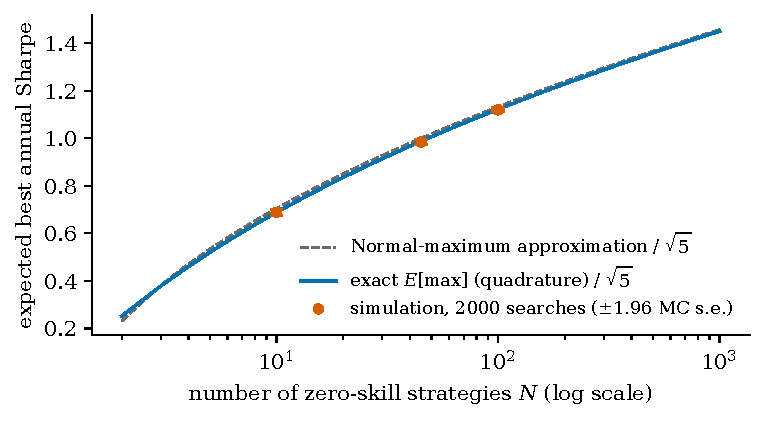
\includegraphics[width=0.78\textwidth]{figures/fig1_best_of_n.pdf}
\caption{Expected best annualized Sharpe ratio among $N$ zero-skill IID Normal strategies over five years of 250 daily returns. Curves: the approximation Eq.~\eqref{eq:emax} and exact quadrature, both divided by $\sqrt5$. Points: D1 simulation, 2000 searches per $N$, $\pm1.96$ Monte Carlo standard errors. The simulation agrees with the exact value; the approximation is 0.016 higher at $N=10$. Source: \texttt{results/best\_of\_n.txt}; curves evaluated analytically.}\label{fig:bestofn}
\end{figure}

\section{Empirical results}\label{sec:results}

Numerical claims in this section are RECOMPUTED from the accompanying outputs; Table~\ref{tab:replication} identifies PAPER values and their source pages. Every rate in this section is a false-pass rate: the share of zero-edge datasets in which a hurdle was passed. A correctly sized 5\% rule passes about 5\% of the time. Bracketed numbers are exact 95\% intervals for that share and measure Monte Carlo error only. ``Detected'' and ``suggestive'' follow the rule in Section~\ref{sec:design}.

\subsection{IID baseline: PSR versus DSR in a search}\label{sec:res:dsr}

PSR ignores the search and DSR is designed to correct for it, so we first measure both on IID data. On a fixed IID Normal strategy (D3), PSR(0)$\,>0.95$ is passed in 4.95\% [4.04, 5.99] of 2000 datasets: the 5\% reading holds at $T=1248$. Applied to the best of 100 zero-skill strategies (D2), PSR(0)$\,>0.95$ is passed in 99.15\% [98.64, 99.50] of searches. DSR$\,>0.95$ is passed in 0.05\% [0.00, 0.28] of D2 searches (1 of 2000) and in 0.00\% [0.00, 0.18] of D3's IID searches, and the winner's mean DSR in D2 is 0.488.

The low DSR rate follows from the 2014 construction. Think of the 100 trial Sharpes as 100 draws, each with a standard error $s=(T-1)^{-1/2}$. The winner's Sharpe is centred near $\SR_0$, so DSR is centred near one half, and DSR exceeds 0.95 only if the winner beats $\SR_0$ by $1.645\,s$. But the best of 100 draws varies much less than any single draw: its standard deviation is $0.43\,s$. The hurdle therefore sits about $1.645/0.43\approx3.9$ standard deviations of the maximum above its mean, and the exact probability of crossing it, with $V$ known, is 0.15\% (Appendix~\ref{app:derivations}). \citet[Exhibit~3, p.~11]{lopezdeprado2026porcu} report 0.1643\% for a stylized location-only rule at $K=100$; our 0.05\% is the rate of the operational procedure with estimated $V$ and plug-in moments. DSR(0.95) is a conservative screen under this null, not a 5\% test, and neither paper claims otherwise.

\subsection{Serial dependence, GARCH, heavy tails and correlation}\label{sec:res:calib}

D3 relaxes one IID assumption at a time, with zero true edge throughout. Table~\ref{tab:calibration} reports every cell and Figure~\ref{fig:calibration} plots the false-pass rates.

\begin{table}[htbp]
\centering\small
\begin{threeparttable}
\footnotesize\setlength{\tabcolsep}{4pt}
\caption{Zero-edge synthetic calibration (D3). False-pass rates in \% with exact 95\% intervals, 2000 datasets per cell. Mean PBO $\pm$ one Monte Carlo s.e., 200 datasets. $N=100$, $T=1248$, $S=16$.}\label{tab:calibration}
\begin{tabular}{@{}lccccc@{}}
\toprule
Scenario & PSR(0)$\,>0.95$ & PSR, Newey--West & DSR, $N=100$ & DSR, $\hat N$ & Mean PBO \\
\midrule
IID Normal & 4.95 [4.04, 5.99] & 5.10 & 0.00 [0.00, 0.18] & & $0.520\pm0.010$ \\
AR(1) $\phi=0.1$ & 6.35 [5.32, 7.51] & 5.30 & 0.10 [0.01, 0.36] & & $0.495\pm0.010$ \\
AR(1) $\phi=0.3$ & 11.85 [10.47, 13.35] & 7.10 [6.01, 8.31] & 0.70 [0.38, 1.17] & & $0.482\pm0.011$ \\
GARCH (0.05, 0.90) & 4.70 [3.81, 5.72] & 4.60 & 0.15 [0.03, 0.44] & & $0.481\pm0.011$ \\
GARCH (0.10, 0.85) & 5.45 [4.50, 6.54] & 5.80 & 0.10 [0.01, 0.36] & & $0.501\pm0.011$ \\
Student-$t$, $\nu=8$ & 4.35 [3.50, 5.34] & 4.65 & 0.15 [0.03, 0.44] & & $0.511\pm0.011$ \\
Student-$t$, $\nu=5$ & 4.85 [3.95, 5.88] & 5.20 & 0.05 [0.00, 0.28] & & $0.504\pm0.011$ \\
Equicorr.\ $\rho=0.3$ & 5.35 [4.40, 6.43] & 5.55 & 0.70 [0.38, 1.17] & 1.05 [0.65, 1.60] & $0.512\pm0.011$ \\
Equicorr.\ $\rho=0.7$ & 4.95 [4.04, 5.99] & 5.20 & 2.60 [1.95, 3.40] & 5.05 [4.13, 6.10] & $0.504\pm0.011$ \\
\bottomrule
\end{tabular}
\begin{tablenotes}\footnotesize
\item PSR is computed on a fixed strategy, DSR on the full-sample winner. $\hat N$ is Eq.~\eqref{eq:impliedn}, only meaningful for correlated designs; its mean is 70.3 at $\rho=0.3$ and 30.7 at $\rho=0.7$. Newey--West uses 7 Bartlett lags. Exact binomial tests of the PSR column against 5\%, Holm over nine scenarios: $\phi=0.3$ detected ($p<10^{-4}$); $\phi=0.1$ suggestive (exact $p=0.0075$, Holm $p=0.060$); all others not different from 5\% (Holm $p=1$). PBO$\,\le0.05$ was passed by a zero-edge set in at most 1 of 200 datasets in any scenario. Source: \texttt{results/calibration.txt}, \texttt{results/manuscript\_numbers.txt}.
\end{tablenotes}
\end{threeparttable}
\end{table}

\begin{figure}[htbp]
\centering
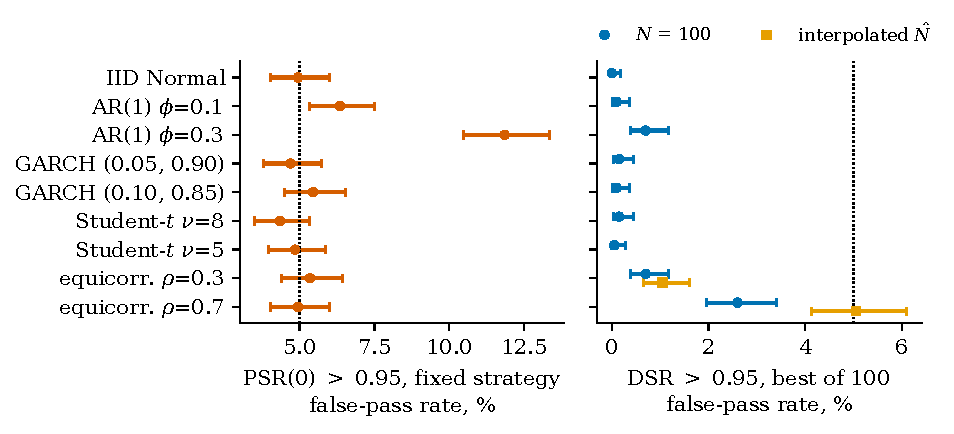
\includegraphics[width=0.92\textwidth]{figures/fig2_calibration.pdf}
\caption{False-pass rates under zero true edge across the D3 scenarios, with exact 95\% intervals (2000 datasets per point). Left: uncorrected PSR(0)$\,>0.95$ on a fixed strategy. Right: DSR$\,>0.95$ on the best of 100, with $N=100$ and, in correlated designs, with the interpolated $\hat N$. Dotted line: 5\%. Only AR(1) moves PSR; only cross-strategy correlation moves DSR materially. Source: \texttt{results/calibration.txt}.}\label{fig:calibration}
\end{figure}
\FloatBarrier

\paragraph{PSR and serial dependence.} H1 fails for AR(1) $\phi=0.3$ (detected), is in doubt for $\phi=0.1$ (suggestive), and is not rejected in the other scenarios at this simulation resolution. The rates agree with Proposition~\ref{prop:rate}: 6.35\% against 6.84\% and 11.85\% against 11.37\%, both inside the simulated intervals (Figure~\ref{fig:psrar1}), so H2 is supported in the synthetic design. GARCH returns are serially uncorrelated, so $F=1$, and at $\SR=0$ the kurtosis term in Eq.~\eqref{eq:mertens} vanishes. The GARCH and Student-$t$ rates near 5\% are therefore what theory predicts at $\SR^\ast=0$; they say nothing about PSR at $\SR^\ast>0$, where kurtosis and volatility clustering do enter. For GARCH(1,1), \citet[Propositions~4.7--4.8]{lopezdeprado2026garch} confirm that the clustering terms vanish at zero mean; both of our GARCH settings satisfy their finite-fourth-moment condition $\alpha^2\kappa_z+2\alpha\beta+\beta^2<1$ (0.9075 and 0.9225 with Gaussian innovations, $\kappa_z=3$).

\paragraph{Newey--West correction.} With 7 Bartlett lags the $\phi=0.3$ rate falls to 7.10\% [6.01, 8.31], not to 5\%. Truncation bias alone, an expected Bartlett factor of 1.704 against the true 1.857, predicts 5.76\%, below the simulated interval; the remaining excess is consistent with sampling noise in $\hat F_b$, which the Normal approximation ignores, and with the known liberality of HAC inference in moderate samples \citep{ledoit2008}. Longer bandwidths, prewhitening, fixed-$b$ critical values \citep{kiefer2005} and the parametric AR(1) correction of \citet[Eq.~2]{lopezdeprado2026lipton}, which matches this process exactly, were not tried. In every other scenario the corrected rate is within its interval of 5\%.

\begin{figure}[htbp]
\centering
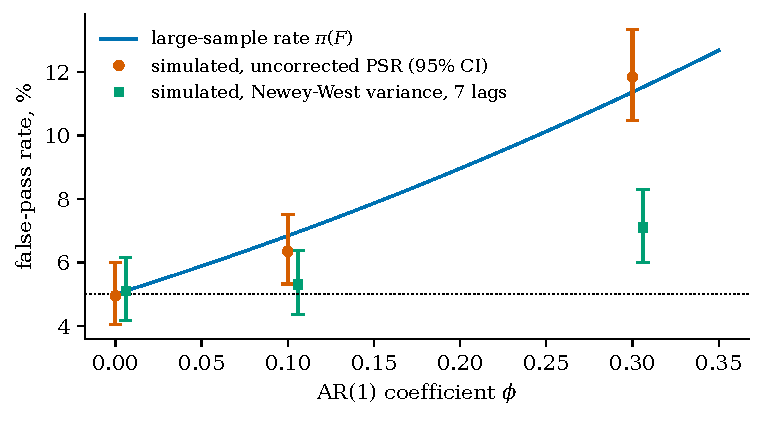
\includegraphics[width=0.78\textwidth]{figures/fig3_psr_ar1.pdf}
\caption{Uncorrected PSR(0)$\,>0.95$ false-pass rate for a zero-Sharpe Gaussian AR(1), $T=1248$. Line: large-sample rate $\pi(F)$ from Eq.~\eqref{eq:ar1rate}. Circles: D3 simulation (2000 datasets each, exact 95\% intervals). Squares: the same datasets with a Newey--West variance (7 lags), shifted right for legibility. Dotted line: 5\%. Source: \texttt{results/calibration.txt}, \texttt{results/psr\_ar1\_curve.txt}.}\label{fig:psrar1}
\end{figure}

\paragraph{DSR and correlated strategies.} H3 fails in the conservative direction: in eight of nine scenarios DSR is passed in at most 0.70\% of searches. The exception is strong cross-strategy correlation. Write returns as $r_{it}=\sqrt{\rho}\,f_t+\sqrt{1-\rho}\,e_{it}$, with a common shock $f_t$ and strategy-specific shocks $e_{it}$. The trial Sharpes share the common shock, so the cross-sectional variance $V$ measures only idiosyncratic dispersion, of order $(1-\rho)/T$. $\SR_0=\sqrt V\,\E[\max_N]$ shrinks, while the winner still carries the common shock, whose variance is of order $\rho/T$. DSR's false-pass rate rises to 2.60\% at $\rho=0.7$ with $N=100$, and to 5.05\% with $\hat N=30.7$. As $\rho\to1$ every trial becomes the same strategy, and DSR tends to PSR(0), whose rate is 5\%. The 5.05\% is where this design happens to cross 5\%, not evidence that Eq.~\eqref{eq:impliedn} recovers a true number of independent trials. For this one-factor design the expected maximum is exactly $\sqrt{1-\rho}$ times the IID value: 1.373 at $N=100$ and $\rho=0.7$ by quadrature, or 1.386 with Eq.~\eqref{eq:emax}, whereas the interpolation with $\hat N=30.7$ and $V=0.3$ gives 1.141 (standardized units). Recovering $\hat N=30.715\pm0.019$ only checks the estimate of Eq.~\eqref{eq:impliedn}. \citet[Appendix~A.3]{lopezdeprado2026lipton} estimate the effective number of trials by clustering or from eigenvalues instead; those estimators were not tested here.

\paragraph{PBO.} H4 holds in every scenario: mean PBO is within about two standard errors of 1/2, and PBO$\,\le0.05$ was passed by a zero-edge set at most once in 200 datasets. This is a sanity check rather than a finding: with exchangeable strategies, symmetry makes one half the expected value, and these nulls do not test the mechanism by which PBO detects overfitting. Paired time-shuffle controls under GARCH give $-0.002\pm0.004$ and $+0.009\pm0.004$.

\paragraph{PBO with one true edge (D5, exploratory).} Under IID noise, mean PBO falls from 0.516 at $\SR_a=0$ to 0.433, 0.189 and 0.026 at $\SR_a=1,2,3$ (Appendix Table~\ref{tab:d5}). Under AR(1) $\phi=0.3$ noise it is higher at $\SR_a=2$ ($0.391\pm0.043$ against $0.189\pm0.037$) and at $\SR_a=3$ ($0.098\pm0.019$ against $0.026\pm0.007$); no change is detected under GARCH. The edge was fixed as a daily mean-to-SD ratio, and under AR(1) the same daily ratio is a weaker signal at the horizon of a CSCV half: the label $\SR_a=2$ corresponds to a Sharpe ratio of 1.47 for 250-day summed returns. That alone can explain much of the shift. Only mean PBO was measured, not the probability of passing PBO$\,\le0.05$ or of selecting the planted strategy, and 20 skewed values per cell make Normal-theory comparisons rough. We draw no conclusion about PBO's power under dependence.

\subsection{Real daily returns: block bootstrap of industry portfolios}\label{sec:res:real}

Synthetic AR(1) is stylized. Here we ask whether the dependence in actual daily returns is large enough to change PSR's false-pass rate (D4). Table~\ref{tab:real} reports every run, Figure~\ref{fig:real} plots them, and Table~\ref{tab:controls} reports the post hoc controls (D8).

\begin{table}[htbp]
\centering\small
\begin{threeparttable}
\caption{PSR(0)$\,>0.95$ false-pass rates on block-bootstrapped industry returns with zero true edge (D4). $T=1248$, 2000 datasets per row, PSR on a uniformly drawn industry. One Holm family of eight tests.}\label{tab:real}
\begin{tabular}{@{}lccccl@{}}
\toprule
Run & Rate, \% [95\% CI] & Approx., \% & Exact $p$ & Holm $p$ & Verdict \\
\midrule
Full window, $L=1$ & 5.35 [4.40, 6.43] & 4.99 & 0.47 & 0.94 & none \\
Full window, $L=5$ & 5.15 [4.22, 6.21] & 5.42 & 0.76 & 0.94 & none \\
Full window, $L=20$ & 6.25 [5.23, 7.40] & 5.50 & 0.014 & 0.096 & suggestive \\
Full window, $L=60$ & 6.25 [5.23, 7.40] & 5.39 & 0.014 & 0.096 & suggestive \\
Replicate, $L=20$ & 5.90 [4.91, 7.02] & 5.50 & 0.072 & 0.217 & none \\
Replicate, $L=60$ & 6.00 [5.00, 7.13] & 5.39 & 0.045 & 0.181 & suggestive \\
\midrule
1971--1998, centred, $L=20$ & 8.35 [7.17, 9.65] & 8.37 & $<10^{-4}$ & $<10^{-4}$ & detected (above) \\
1999--2026, centred, $L=20$ & 3.85 [3.05, 4.79] & 3.94 & 0.018 & 0.096 & suggestive (below) \\
\bottomrule
\end{tabular}
\begin{tablenotes}\footnotesize
\item Approximation: $\pi(F^{\mathrm{boot}})$ from Eq.~\eqref{eq:blockF} with each industry's circular autocorrelations, averaged over industries. The approximations include the partial-final-block correction; the superseded output is preserved separately. Sub-period counts are 167/2000 and 77/2000. Holm $p$ over all eight rows from \texttt{results/review\_checks.txt}; an earlier version split the rows into three families and labelled the 1999--2026 row detected. Sources: \texttt{results/french\_bootstrap.txt}, \texttt{french\_followups.txt}, \texttt{g6\_corrected.txt}, \texttt{review\_checks.txt}.
\end{tablenotes}
\end{threeparttable}
\end{table}

\begin{figure}[htbp]
\centering
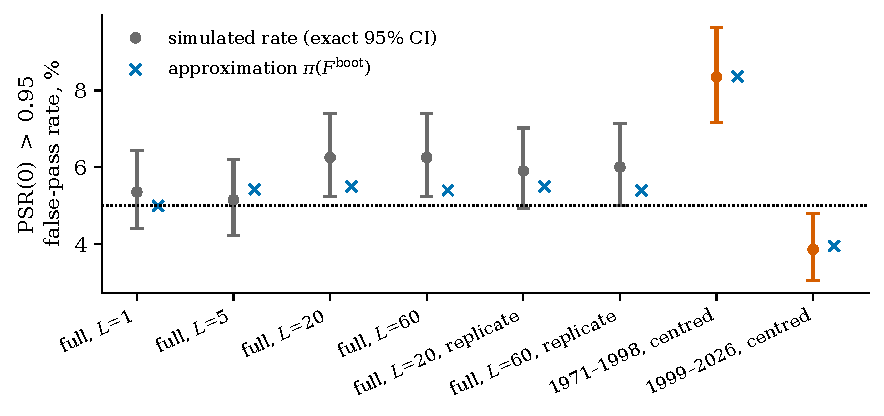
\includegraphics[width=0.85\textwidth]{figures/fig4_real_data.pdf}
\caption{PSR(0)$\,>0.95$ false-pass rates on block-bootstrapped daily industry returns with zero true edge (D4), with exact 95\% intervals (2000 datasets per point). Crosses: the approximation $\pi(F^{\mathrm{boot}})$, Eqs.~\eqref{eq:ar1rate}--\eqref{eq:blockF}. The two right-hand points resample each period after centring each industry within that period. Intervals are Monte Carlo error given the observed history. Source: \texttt{results/french\_bootstrap.txt}, \texttt{french\_followups.txt}, \texttt{g6\_corrected.txt}.}\label{fig:real}
\end{figure}

\paragraph{Full history versus sub-periods.} On the full 1971--2026 history the excess over 5\% is at most suggestive: 6.25\% at $L=20$ and 60, and 5.90\% and 6.00\% in the replicate. Mean daily lag-1 autocorrelation across industries was $+0.157$ in 1971--1998, positive in all 49 industries, and $-0.026$ in 1999--2026. Resampling the early period with each industry centred, PSR passes 8.35\% [7.17, 9.65]; resampling the late period it passes 3.85\% [3.05, 4.79]. The early excess is detected; the late shortfall is suggestive once the eight rows are treated as one Holm family. The full-window rate is close to the simple average of the two (6.1\%), so the full-window figure describes neither period.

\paragraph{Why the rates differ (post hoc controls).} Removing the dependence while keeping each period's returns ($L=1$) brings both periods back to 5\%: 5.05\% [4.39, 5.77] and 4.67\% [4.04, 5.38] (Table~\ref{tab:controls}). Fat tails, volatility levels and the random choice of industry therefore do not create the contrast; time-series dependence does. Filtering out linear autocorrelation (AR(5) residuals) removes most but not all of the early excess: 5.97\% [5.26, 6.75] remains, so some nonlinear dependence or residual short-range structure also matters. The direction of the late-period shortfall is stable: across 200 resampled histories of each period the predicted rate stays in [7.53, 9.07]\% for 1971--1998 and in [3.54, 4.26]\% for 1999--2026, below 5\% in every resample, and it keeps both signs for split dates from 1993 to 2004. A fixed correction calibrated on one period would be wrong in the other.

\begin{table}[htbp]
\centering\small
\begin{threeparttable}
\caption{Post hoc controls for the sub-period result (D8), PSR(0)$\,>0.95$ false-pass rates in \%.}\label{tab:controls}
\begin{tabular}{@{}lcc@{}}
\toprule
Check & 1971--1998 & 1999--2026 \\
\midrule
Main result, $L=20$ (Table~\ref{tab:real}) & 8.35 [7.17, 9.65] & 3.85 [3.05, 4.79] \\
Dependence removed, $L=1$ (4000 datasets) & 5.05 [4.39, 5.77] & 4.67 [4.04, 5.38] \\
AR(5) residuals, $L=20$ (4000 datasets) & 5.97 [5.26, 6.75] & 5.58 [4.88, 6.33] \\
Predicted rate, 95\% range, 200 histories & [7.53, 9.07] & [3.54, 4.26] \\
Predicted rate, split in 1993 / 1996 / 2001 / 2004 & 8.96 / 8.70 / 7.81 / 7.31 & 4.10 / 4.08 / 3.92 / 3.79 \\
\bottomrule
\end{tabular}
\begin{tablenotes}\footnotesize
\item Resampled histories: 250-day block resamples of each period, re-centred, predicted rate at $L=20$. Source: \texttt{results/review\_checks.txt}.
\end{tablenotes}
\end{threeparttable}
\end{table}

\paragraph{Status of this result.} The sub-period analysis was designed after the full-window results were seen. Its first run resampled the periods without centring them; that run disagreed with the approximation (10.45\% simulated against 8.38\% predicted, $z=+3.34$), the cause was traced to nonzero period means, and the run was withdrawn (Appendix~\ref{app:corrections}). The recorded prediction for the corrected run equals the approximation and was proposed after the uncentred run was seen, and the agreement between them (within 0.1 points) checks only the Normal approximation, since Eq.~\eqref{eq:blockF} is the exact variance of the same bootstrap. The intervals are Monte Carlo error given one history and one bootstrap design. We therefore treat the early excess as established for this design, and the late shortfall as likely but not established at the 5\% familywise level.

\paragraph{Corrections and controls in the full window.} A Newey--West variance on the replicate datasets gives 5.60\% and 5.70\% at $L=20$ and 60, and AR(5) residuals give 5.30\% and 5.35\%; all intervals contain 5\%. These are robustness checks, not isolated interventions, because residual filtering also changes marginal moments and cross-industry relationships. Weekly five-day sums give 4.35\% [3.50, 5.34] but change the horizon, sample span and moments at once.

\paragraph{DSR and PBO on industries.} DSR's false-pass rate stays below 5\% throughout: 3.05--3.55\% with $\hat N$ (mean 23.0--23.3 for 49 industries) and 1.25--1.90\% with $N=49$. Mean PBO is 0.505--0.520 against the reference $25/49=0.510$, with Monte Carlo standard errors of 0.012--0.014 (Appendix Table~\ref{tab:d4extra}). A time-shuffle control gave $+0.017\pm0.005$ at $L=60$ in the first run; it did not replicate in 400 further datasets ($+0.001\pm0.004$ with fixed block positions, $-0.001\pm0.004$ with random positions).

\paragraph{Alternative explanation.} The pre-1999 autocorrelation is plausibly in part an effect of nonsynchronous trading in portfolio returns \citep{lo1990}, and its decline coincides with the rise in liquidity and fall in tick sizes documented by \citet{chordia2005,chordia2008}. Whatever its source, it is real dependence in the series to which PSR is applied, though not necessarily exploitable predictability. We did not test the mechanism.

\subsection{Strategy-search case study}\label{sec:res:case}

DSR and PBO are commonly reported for parameter searches, but neither compares the winner with the market. D6 tests H5: whether the best of 93 moving-average settings beats buy-and-hold once dependence and the search are accounted for. The predictions recorded before the run were PBO between 0.05 and 0.5, DSR above 0.95, PBO roughly unchanged across costs, and an in-sample Sharpe above the market's. The first, second and fourth were correct; the third was not judged because no tolerance was set in advance. Table~\ref{tab:case} reports the search, and Table~\ref{tab:bench} the market tests.

\begin{table}[htbp]
\centering\small
\begin{threeparttable}
\caption{Strategy search on the US market factor (D6). 93 settings, 18 July 1972 to 30 September 2026, $T=13{,}664$. Sharpe ratios annualized by $\sqrt{250}$.}\label{tab:case}
\begin{tabular}{@{}lccc@{}}
\toprule
Cost per change in position & 0 bps & 5 bps (main) & 10 bps \\
\midrule
Selected setting (fast/slow) & 15/225 & 15/225 & 15/225 \\
Its Sharpe ratio & 0.593 & 0.588 & 0.582 \\
Buy-and-hold Sharpe ratio & 0.458 & 0.458 & 0.458 \\
Settings above buy-and-hold & 55 of 93 & 50 of 93 & 45 of 93 \\
PSR(0) of the selected setting & 1.0000 & 1.0000 & 1.0000 \\
DSR, $N=93$ & 0.9985 & 0.9980 & 0.9969 \\
DSR, $\hat N=17.2$ & 0.9995 & 0.9994 & 0.9991 \\
PBO ($S=16$) & 0.240 & 0.208 & 0.193 \\
\bottomrule
\end{tabular}
\begin{tablenotes}\footnotesize
\item Source: \texttt{results/ma\_crossover.txt}.
\end{tablenotes}
\end{threeparttable}
\end{table}

\paragraph{Search-adjusted statistics against zero skill.} The winner's DSR is 0.998 with $N=93$ and 0.999 with $\hat N=17.2$: its Sharpe is far above $\SR_0$, the expected best of 93 zero-skill trials. Over 54 years of daily data the standard error of a daily Sharpe is about $(13{,}664)^{-1/2}\approx0.0086$, and the 93 settings are closely related, so $V$ and $\SR_0$ are small; a mostly-long rule can earn the equity premium and clear a zero-skill benchmark without adding value relative to the market. With $V$ fixed, DSR falls below 0.95 only at $N\approx7.4\times10^5$ trials (Figure~\ref{fig:dsrn}). PBO is 0.208: in 20.8\% of the 12,870 CSCV splits, the IS winner ranked at or below the OOS median of the 93 settings. That fails the customary 0.05 cut-off, but PBO is fragile here: building the same signals from the market's excess-return index instead of its total-return index changes the winner to 5/200 and PBO to 0.051 (Table~\ref{tab:robust}).

\begin{table}[htbp]
\centering\small
\begin{threeparttable}
\caption{The selected setting (15/225, 5 bps) judged against different benchmarks.}\label{tab:bench}
\begin{tabularx}{\textwidth}{@{}>{\raggedright\arraybackslash}p{4.6cm}>{\raggedright\arraybackslash}X>{\raggedright\arraybackslash}p{4.4cm}@{}}
\toprule
Question & Selected setting & Over all 93 settings \\
\midrule
Better than the best of 93 zero-skill trials? & DSR 0.998 & n/a \\
Positive active-return Sharpe after deflation? & DSR of (setting $-$ market) 0.030 & n/a \\
Higher Sharpe ratio than the market? & $+0.130$ (s.e.\ 0.099), 95\% CI [$-0.064$, 0.323], one-sided $p=0.094$ & Bonferroni: 0 of 93 pass; SPA $p=0.504$ \\
\quad with 0 / 44 HAC lags & $p=0.105$ / 0.100 & Bonferroni: 0 of 93 at either \\
\quad bootstrap, block 20 / 250 & $p=0.105$ / 0.099 & \\
Return beyond market exposure (alpha)? & $\beta=0.510$; alpha 3.16\%/yr, $t=2.71$, one-sided $p=0.0033$ & Bonferroni: 0 of 93 pass; 33 of 93 have $t>1.645$; SPA $p=0.045$ \\
\quad SPA, other blocks$^{a}$ & & $p=0.046$ / 0.065 / 0.035 / 0.047 \\
\bottomrule
\end{tabularx}
\begin{tablenotes}\footnotesize
\item $^{a}$Mean blocks 5, 60 and 250 days, and 20 days with a second seed. HAC tests use 11 Bartlett lags. The bootstrap rows are studentized stationary bootstraps. The unadjusted $p$-values of the selected setting are selection-biased: it has the smallest of the 93. The alpha tests, the market-benchmarked DSR, the studentized bootstrap and the alpha SPA are post hoc (D8); the alpha SPA was chosen after the alpha $t$-statistics were seen. Sources: \texttt{results/market\_comparison.txt}, \texttt{manuscript\_numbers.txt}, \texttt{case\_study\_checks.txt}, \texttt{review\_checks.txt}.
\end{tablenotes}
\end{threeparttable}
\end{table}

\paragraph{Against the market.} Table~\ref{tab:bench} answers three questions about the same setting. First, DSR of active returns (the setting's return minus the market's, with $V$ from the 93 active-return Sharpes) is 0.030. This changes the return variable and its volatility, moments and trial dispersion; it is not a deflation of $\hSR_x-\hSR_y$ or a test of regression alpha. A low active-return DSR therefore does not resolve either of those nulls. Second, the Sharpe advantage of $+0.130$ is not significant: 43 of 93 differences are negative (Figure~\ref{fig:grid}), the largest $z$ is 1.31 (Figure~\ref{fig:z}), no setting passes Bonferroni, and Hansen's SPA, which accounts for the correlation between settings, gives $p=0.504$. Third, the setting's market-adjusted return is stronger: with a market beta of 0.51 it earns an alpha of 3.16\% a year ($t=2.71$). That passes for 0 of 93 settings under Bonferroni, but Hansen's SPA on the 93 alphas gives $p=0.045$, and between 0.035 and 0.065 across bootstrap block lengths. For the baseline idealized execution convention the alpha evidence is therefore borderline and exploratory. With 2000 bootstrap draws, a $p$-value near 0.05 has Monte Carlo s.e. about 0.005; the test was chosen after the alpha $t$-statistics were seen. H5 is not rejected for the Sharpe ratio; for market-adjusted return the baseline evidence is suggestive, but sensitive to execution delay.

\paragraph{Power.} Holding the estimated standard error of the Sharpe difference fixed, a Normal approximation gives 80\% power for a single one-sided 5\% test only against a true difference of 0.246, and for the Bonferroni test only against 0.406. Against a true difference of 0.130 the implied power is 0.37 unadjusted and 0.025 after Bonferroni. These are calculations for the selected setting's test, not the measured power of the whole search-and-selection procedure. At a common volatility of 16.9\% a year, a Sharpe difference of 0.130 corresponds to about 2.2\% a year of mean excess return. This is a hypothetical volatility-normalized comparison, not the observed return advantage: the rule has lower volatility and a lower arithmetic total return than the market (Appendix Table~\ref{tab:perf}). The observed Sharpe test cannot resolve an advantage of this size reliably.

\begin{figure}[htbp]
\centering
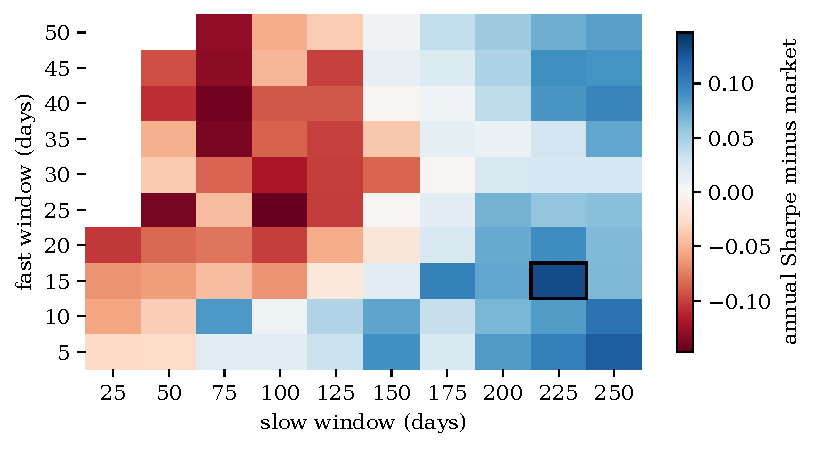
\includegraphics[width=0.8\textwidth]{figures/fig5_grid.pdf}
\caption{Annualized Sharpe ratio of each moving-average setting minus that of buy-and-hold, 5 bps, 1972--2026 (D6). The boxed cell is the in-sample winner, 15/225. Blank cells have fast $\ge$ slow. Positive differences cluster at long slow windows, which stay long the market on most days. Source: \texttt{results/market\_comparison.txt}.}\label{fig:grid}
\end{figure}

\begin{figure}[htbp]
\centering
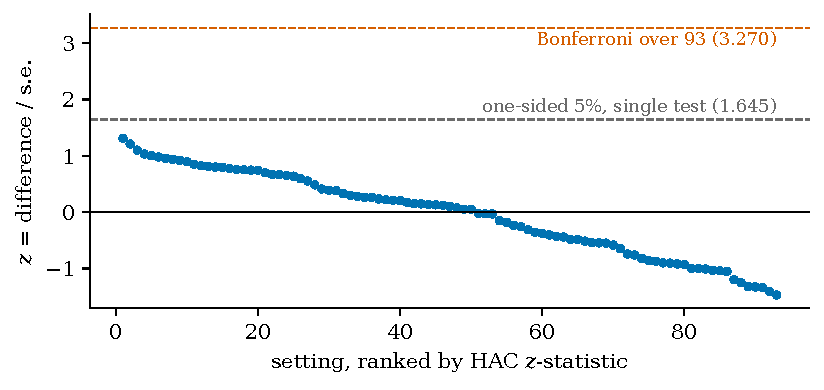
\includegraphics[width=0.8\textwidth]{figures/fig6_z.pdf}
\caption{Paired HAC $z$-statistics (11 Bartlett lags) of the Sharpe difference for all 93 settings against buy-and-hold, ranked. The largest is 1.31 (setting 15/225); the Bonferroni threshold at family level 5\% is 3.270. Source: \texttt{results/market\_comparison.txt}.}\label{fig:z}
\end{figure}

\section{Robustness and sensitivity}\label{sec:robust}

All checks in this section are exploratory or post hoc (Table~\ref{tab:classification}). They use 5 bps and 11 lags unless stated; Table~\ref{tab:robust} reports them.

\begin{table}[htbp]
\centering\small
\begin{threeparttable}
\caption{Case-study robustness (D7, D8). Annualized Sharpe ratios and differences; paired tests with 11 Bartlett lags.}\label{tab:robust}
\begin{tabularx}{\textwidth}{@{}>{\raggedright\arraybackslash}p{4.3cm}>{\raggedright\arraybackslash}X@{}}
\toprule
Check & Result \\
\midrule
Baseline (signal acts next day) & 15/225: Sharpe 0.588 vs 0.458; PBO 0.208; DSR 0.9980; difference $+0.130$, $p=0.094$ \\
One extra day of execution lag & 15/225 still selected: Sharpe 0.578; PBO 0.216; DSR 0.9959; difference $+0.120$ (s.e.\ 0.099), $p=0.113$; 48 of 93 above market \\
Signal on the excess-return index (D8) & Winner changes to 5/200: Sharpe 0.626; PBO 0.051; difference $+0.168$ (s.e.\ 0.112, $z=1.50$); 39 of 93 above market; 15/225 falls to 0.467 \\
Turnover of 15/225 & 72 position changes in 13,664 trading days (about 54 years), 1.32 per 250-day year; long on 76\% of days \\
Break-even cost & 121 bps per change before its Sharpe equals the market's \\
1972--1998 (6,686 days) & Sharpe 0.568 vs 0.500; difference $+0.068$ (s.e.\ 0.134), $p=0.305$ \\
1999--2026 (6,978 days) & Sharpe 0.606 vs 0.439; difference $+0.167$ (s.e.\ 0.140), $p=0.117$ \\
DSR break-even trial count & DSR $<0.95$ only for $N\gtrsim7.4\times10^5$, $V$ fixed \\
Walk-forward, 1982--2026 & Re-selected each January on all prior data: OOS Sharpe 0.466 vs market 0.536; difference $-0.070$ (s.e.\ 0.107), one-sided $p=0.74$; 10 distinct settings chosen \\
Same window, fixed settings (hindsight, D8) & Fixed 15/225: 0.649; median of 93: 0.546; 50 of 93 above the market \\
\bottomrule
\end{tabularx}
\begin{tablenotes}\footnotesize
\item Sources: \texttt{results/case\_study\_checks.txt}, \texttt{performance\_checks.txt}, \texttt{review\_checks.txt}. The walk-forward sample (11,276 days) differs from the full sample, so its market Sharpe differs from 0.458.
\end{tablenotes}
\end{threeparttable}
\end{table}

\paragraph{Execution lag and costs.} The selected rule trades about 1.3 times a year. One additional day of delay lowers its Sharpe by 0.010 and leaves it the winner, and costs between 0 and 10 bps move its Sharpe by 0.011. These checks do not change the inconclusive standalone Sharpe comparison. A further post hoc check of all 93 alphas with this extra delay gives SPA $p=0.084$ (2000 joint stationary-bootstrap draws, mean block 20 days, seed 20261118; Monte Carlo s.e. 0.0062). The selected rule still has alpha 3.02\% a year and HAC $t=2.56$, but the family test does not reject at 5\%. Thus the baseline borderline alpha evidence is sensitive to execution timing and does not establish implementability. The complete 93-rule table and bootstrap vectors are preserved with the review evidence. The two $p$-values alone do not test the effect of delay; the delayed result is a sensitivity check, not proof that alpha disappears. The break-even cost of 121 bps per change is large compared with a flat 5--10 bps charge, but the cost model ignores market impact, financing and taxes.

\paragraph{Signal construction.} The choice of index from which the moving averages are computed matters more than lag or costs. With the total-return index, which includes the risk-free rate, 15/225 wins; with the excess-return index, 5/200 wins, PBO drops from 0.208 to 0.051, and 15/225 itself falls to a Sharpe of 0.467. The market-test conclusion does not change ($z=1.50$ for the new winner), but the identity of the winner and the PBO verdict are not properties of the data alone.

\paragraph{Lag specification and bootstrap.} The HAC standard error of the Sharpe difference is 0.104 with 0 lags, 0.099 with 11 and 0.101 with 44, and a studentized stationary bootstrap gives $p=0.105$ and 0.099 for mean blocks of 20 and 250 days, close to the Normal $p$ of 0.094. The market factor's daily lag-1 autocorrelation over the sample is $-0.001$.

\paragraph{Sub-periods.} The in-sample advantage is larger after 1999 ($+0.167$) than before ($+0.068$), so the pre-1999 stale-price autocorrelation of Section~\ref{sec:res:real} does not explain it. Neither difference is significant, and each has a standard error of about 0.14.

\paragraph{Walk-forward selection.} Re-selecting the setting each January from past data alone, with costs charged on the positions actually held, gives an out-of-sample Sharpe of 0.466 over 1982--2026 against the market's 0.536 on the same days: a difference of $-0.070$ (s.e.\ 0.107), well within noise. This tests the rule ``hold last period's best setting'', not the rule family. Over the same days, the fixed setting 15/225 has a Sharpe of 0.649 and 50 of 93 fixed settings beat the market, but those figures use hindsight. The walk-forward design was not logged before it ran.

\begin{figure}[htbp]
\centering
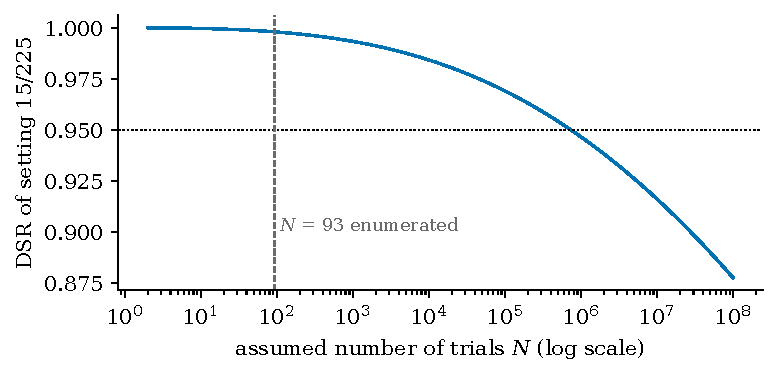
\includegraphics[width=0.78\textwidth]{figures/fig7_dsr_vs_n.pdf}
\caption{DSR of setting 15/225 as a function of the assumed number of trials $N$, holding the observed $V$, skewness, kurtosis and $T=13{,}664$ fixed. Dotted line: 0.95. Dashed line: the 93 settings actually tried. Evaluated from Eqs.~\eqref{eq:psr}--\eqref{eq:dsr}; source: \texttt{results/fig7\_dsr\_vs\_n.txt}.}\label{fig:dsrn}
\end{figure}

\section{Discussion}\label{sec:discussion}

\paragraph{Why the case-study statistics disagree.} The four answers in the introduction are consistent once each is matched to its benchmark. DSR 0.998 says the winner beats noise, which a mostly-long rule can do by earning the equity premium. DSR of active returns does not clear its zero-skill screen. This concerns $\SR(x-y)$, whereas the paired test concerns $\SR(x)-\SR(y)$ and alpha adjusts for market exposure. The Sharpe comparison is also inconclusive, and the power calculation shows it had little chance of detecting an edge of about 2\% a year (power 0.37 before, and 0.025 after, the Bonferroni adjustment). The alpha test asks about return beyond constant linear market exposure, with a potential portfolio interpretation under fixed population moments and unconstrained allocation, and gives borderline evidence under baseline execution, which weakens under an extra day of delay. PBO 0.21 says the ranking among 93 similar rules is unstable, and that verdict itself depends on how the signal is constructed. Table~\ref{tab:decision} maps decisions to statistics.

\begin{table}[htbp]
\centering\small
\caption{Which statistic answers which question.}\label{tab:decision}
\begin{tabularx}{\textwidth}{@{}>{\raggedright\arraybackslash}p{3.4cm}>{\raggedright\arraybackslash}p{2.6cm}>{\raggedright\arraybackslash}X>{\raggedright\arraybackslash}X@{}}
\toprule
Decision & Statistic & A pass does not imply & Evidence still needed \\
\midrule
Is one pre-specified Sharpe above a hurdle? & PSR($\SR^\ast$) & Robustness to serial dependence (Secs.~\ref{sec:res:calib}, \ref{sec:res:real}) & HAC or parametric variance, or lower frequency, checked for the period \\
Is a search winner better than the best of $N$ noise trials? & DSR (2014) & A 5\% error rate; skill relative to a benchmark & A defensible $N$; the benchmark that matches the decision \\
Do the search's rankings persist out of sample? & PBO & A probability of future loss & A reference distribution for the rule family; sensitivity to implementation \\
Should capital move to the strategy? & None of the above & & Search-aware tests of Sharpe ratio and alpha against the benchmark, with power; held-out evidence; costs and capacity \\
\bottomrule
\end{tabularx}
\end{table}

\paragraph{Why the methods behave differently.} At true $\SR=\SR^\ast=0$, under the central-limit and consistency conditions above, the leading asymptotic distortion of PSR is governed by the long-run variance of the sample mean. Heavy tails and volatility clustering can still affect finite-sample behavior and whether these conditions hold. Autocorrelation produced the material distortions in the designs studied here. DSR's benchmark is a location shift of a single-strategy distribution, so its size depends on how the spread of the maximum compares with the spread of one estimate, and on how much common variation $V$ misses. CSCV compares relative ranks within a set. Shared return shocks do not generally cancel exactly in finite-sample Sharpe rankings, and mean PBO alone does not identify skill or decision power.

\paragraph{Financial interpretation.} The moving-average rule mainly reduces exposure during long declines: it is long on 76\% of days and has lower volatility than the market (12.1\% against 16.9\% a year, Appendix Table~\ref{tab:perf}). Its estimated positive alpha with beta 0.51 describes performance beyond a constant linear market exposure; it does not identify a causal timing advantage or exclude omitted risk exposures. Our in-sample evidence is weaker than that of \citet{sullivan1999}, whose best Dow Jones rule survived a data-snooping adjustment in sample before failing out of sample, and the walk-forward result here shows only that re-selecting the best setting each year does not reliably capture the in-sample advantage.

\paragraph{Practical consequences.} Four rules follow for a research process. First, check the autocorrelation of PSR's inputs over the period used: the same industry data give a false-pass rate of 8.35\% or 3.85\% depending on the period, and a Newey--West correction removes most but not all of the AR(1) distortion. Second, choose the DSR benchmark to match the decision, in the spirit of the stage-specific nulls of \citet[Exhibit~8]{lopezdeprado2026lipton}: zero skill for ``is this more than noise'', and active returns for an unscaled replacement comparison. DSR of active returns does not replace a Sharpe-difference or alpha test. Third, for long-biased timing rules, test alpha as well as the Sharpe ratio, because the two answer different allocation questions and can disagree. Fourth, report PBO as rank stability, and check its sensitivity to implementation choices before reading it against a cut-off.

\paragraph{Comparison with prior literature.} The AR(1) result confirms \citet{lo2002}, \citet[Remark~3.1]{ledoit2008} and the closed form of \citet[Eq.~2]{lopezdeprado2026lipton}. The IID DSR result reproduces, for the operational 2014 procedure, the conservatism that \citet{lopezdeprado2026porcu} establish for its location-only form. The period effect is consistent with the decline in short-horizon predictability documented by \citet{chordia2008}; its measured consequence for PSR's size appears to be new. The case-study conclusions are in line with the mixed evidence on technical rules \citep{park2007,bajgrowicz2012}. The 2026 papers recommend procedures (DSR-LS and DSR-EO, the AR(1)-corrected variance, clustered effective trials, stage-specific nulls) that may remove the distortions documented here; testing them is outside this paper.

\paragraph{What the results do not establish.} They do not establish the size of PSR at $\SR^\ast>0$, the behaviour of MinTRL under dependence, the power of PBO, the performance of the 2026 DSR variants, a profitable or implementable strategy, or anything about future returns.

\section{Limitations}\label{sec:limits}

\begin{itemize}
\item \textbf{Dataset representativeness.} Real-data results use one vendor's US industry and market portfolios over 1971--2026. Other markets, frequencies or individual securities, and strategy returns rather than portfolio returns, may show different dependence.
\item \textbf{Regime changes.} Dependence is not stable over time. A bootstrap with fixed block length assumes stationarity within the resampled window, is not itself stationary across block positions, and removes dependence beyond $L$. Block lengths were fixed by design, not chosen by a data-driven rule such as \citet{politis2004}.
\item \textbf{Data construction.} The French portfolios are built from CRSP, which includes delisted firms, so survivorship is not a concern at the portfolio level. The research factors use today's vintage of CRSP data and the library's current methodology; they are not the point-in-time series a trader could have observed, and revisions change history.
\item \textbf{Model assumptions.} Synthetic parameter levels are our choices. PSR was tested only at $\SR^\ast=0$. HAC inference requires stationarity, mixing and finite moments that the market history may violate (raw kurtosis 17.7).
\item \textbf{Exploratory, post hoc and multiple analyses.} The hypotheses, the evidence rule, the sub-period design, its prediction, the robustness checks and the review-stage checks were all fixed after earlier results were known. The paper reports well over 100 tests with Holm adjustment only within tables; the alpha SPA was chosen after the alpha $t$-statistics were seen.
\item \textbf{No prospective validation.} All tests use historical data. The walk-forward check is pseudo-out-of-sample on one path, with a rule family chosen with knowledge of the literature.
\item \textbf{Monte Carlo resolution.} With 2000 datasets, effects below about one percentage point in a rate are not resolved; the full-window excesses of 0.4--0.5 points predicted by the approximation had low power to be detected. PBO cells use 200 datasets and D5 only 20.
\item \textbf{Strategy realism.} Same-close fills on a research portfolio, flat costs, and no capacity, financing or tax effects. The case study is a statistical illustration, not an implementable strategy.
\item \textbf{Literature access.} The three 2026 papers were read in the versions listed in the references; their supplementary proofs were not checked. Mertens (2002) and Memmel (2003) were not examined directly, and several later references were read at abstract level only (noted in the bibliography).
\item \textbf{Novelty.} The serial-dependence mechanism, its AR(1) correction, the conservatism of the location-only DSR, the SPA test and the technical-rule evidence are all published. The contribution is replication, operating characteristics in specific designs, the period dependence of PSR's size on real data, and the benchmark comparison in one case study.
\end{itemize}

\section{Data, code and reproducibility}\label{sec:repro}

The earlier clean-environment reproduction is preserved in the review record. A fresh isolated environment with newly installed dependencies was also used for the final checks; the exact command log and comparison scope are in the accompanying reproducibility report. The current \texttt{french\_followups.txt} includes the partial-final-block correction. Its superseded raw output is retained separately: three displayed approximations changed by 0.0001 and two displayed $z$-statistics changed by 0.01, with every simulated count unchanged. The corrected walk-forward output and its original are stored separately. The final test-suite outcome is recorded in the accompanying reproducibility report. Both input archives are identified by SHA-256 and have independently retrieved, hash-verified Internet Archive copies (Appendix~\ref{app:repro}). The data are not redistributed with the code and are not covered by its MIT licence.

\section{Conclusion}\label{sec:conclusion}

How often do standard backtest hurdles pass strategies with no edge when their assumptions fail, and does a historically superior rule survive selection-aware testing? For the first question, the replicated results confirm what theory and recent work predict: uncorrected PSR passes too often under AR(1) dependence, at the rate long-run-variance theory gives, and the 2014 DSR is far from a 5\% test under independent zero-skill searches. On daily US industry returns, PSR's false-pass rate follows the period's dependence: clearly above 5\% in 1971--1998 and probably below it in 1999--2026. DSR becomes less conservative as strategies become correlated. For the second question, the answer depends on the benchmark. The best of 93 moving-average rules clears a zero-skill DSR easily, has no standalone Sharpe advantage established by the tests we ran, and shows baseline market alpha with borderline post hoc search-aware evidence that does not pass at 5\% under an extra day of execution delay. A high value on one of these statistics is not evidence of an investable edge; the benchmark has to match the decision. Nothing here bears on future performance.

\section*{Statements}
\textbf{Data availability.} Kenneth R.\ French Data Library, daily 49 Industry Portfolios and Fama--French research factors, 202609 CRSP release, downloaded 12 November 2026; SHA-256 and archived copies in Appendix~\ref{app:repro}. \textbf{Code availability.} The accompanying repository (MIT licence); the exact commit is recorded with any public release. \textbf{Funding and conflicts of interest.} None declared. \textbf{Ethics.} Not applicable: public aggregate data, no human subjects. \textbf{Assistance and responsibility.} AI tools assisted code review, literature checks, editing and internal adversarial review. Their reports are not independent human peer review; the author retains responsibility for verifying the submission. \textbf{Review status.} The paper has not been peer reviewed.

\bibliographystyle{plainnat}
\bibliography{references}

\appendix

\section{Derivations}\label{app:derivations}

\paragraph{Proposition~\ref{prop:rate}.} Write $\hSR=\bar r/\hat\sigma$. Under $\mu=0$, $\sqrt T\bar r/\sigma\to\mathcal N(0,F)$ by a central limit theorem for stationary weakly dependent sequences, and $\hat\sigma\to\sigma$ in probability, so $\sqrt T\hSR\to\mathcal N(0,F)$ by Slutsky's theorem. Since $\hSR\to0$, the PSR denominator in Eq.~\eqref{eq:psr} tends to 1 and $\sqrt{(T-1)/T}\to1$; hence the PSR $z$-statistic converges to $\mathcal N(0,F)$ and $\Pr(z>z_{1-\alpha})\to1-\Phi(z_{1-\alpha}/\sqrt F)$. For AR(1), $\sum_{k\ge1}\phi^k=\phi/(1-\phi)$, so $F=1+2\phi/(1-\phi)=(1+\phi)/(1-\phi)$. At $\phi=0.3$: $F=1.857$, $1.645/\sqrt{1.857}=1.207$ and $\pi=11.37\%$.

\paragraph{Block-bootstrap factor, Eq.~\eqref{eq:blockF}.} A circular block of length $n$ starting at a uniformly random position $s$ consists of source values $x_{s},\dots,x_{s+n-1}$ (indices modulo the source length $n_0$). Averaging over $s$, $\E[(\sum_{j}\tilde x_{s+j})^2]=n_0^{-1}\sum_s(\sum_j\tilde x_{s+j})^2=n\hat\sigma^2+2\sum_{h=1}^{n-1}(n-h)\hat\gamma^{\circ}_h$, with $\hat\gamma^\circ_h$ the circular sample autocovariance of the centred source. Dividing by $n\hat\sigma^2$ gives $F_n$. Independent block starts make block sums independent with mean zero, so the variance of the total is the sum over $m$ full blocks and one partial block of length $r$; dividing by $T\hat\sigma^2$ gives Eq.~\eqref{eq:blockF}. This is exact for the variance of the bootstrap mean; turning it into a false-pass rate through $\pi(\cdot)$ remains a Normal approximation.

\paragraph{Sharpe-difference influence, Eq.~\eqref{eq:influence}.} $\SR=g(m_1,m_2)=m_1/\sqrt{m_2-m_1^2}$ with $m_1=\E r$ and $m_2=\E r^2$. The gradient is $(\sigma^2+\mu^2,\,-\mu/2)/\sigma^3$. Applying it to the centred moment contributions $(r_t-m_1,\,r_t^2-m_2)$ and simplifying gives $h_t=z_t-\tfrac{\SR}{2}(z_t^2-1)$. For two series the influence of the difference is $h_{x,t}-h_{y,t}$, and its long-run variance divided by $T$ is the asymptotic variance of $\hSR_x-\hSR_y$. This is algebraically equivalent to the four-moment delta method of \citet[Eqs.~1--5]{ledoit2008} and avoids forming a $4\times4$ covariance of raw second moments.

\paragraph{Equicorrelated maximum.} If $X_i=\sqrt\rho Z_0+\sqrt{1-\rho}Z_i$ with IID standard Normals, then $\max_iX_i=\sqrt\rho Z_0+\sqrt{1-\rho}\max_iZ_i$ and $\E\max_iX_i=\sqrt{1-\rho}\,\E[\max_N]$. The cross-sectional variance of the $X_i$ has expectation $1-\rho$, so $\sqrt{V}\E[\max_N]$ targets the right location, but the winner keeps $\sqrt\rho Z_0$, whose variance is $\rho$. This is why DSR's false-pass rate rises with $\rho$. With $N=100$ and $\rho=0.7$: $\sqrt{0.3}\times2.5076=1.373$ (exact), $\sqrt{0.3}\times2.5306=1.386$ (Eq.~\ref{eq:emax}), and $\sqrt{0.3}\,\E[\max_{30.7}]=1.141$ with the interpolated $\hat N$.

\paragraph{Spread of the maximum (Section~\ref{sec:res:dsr}).} For 100 IID standard Normals, quadrature gives mean 2.5076 and standard deviation 0.4294. DSR$\,>0.95$ with $V$ known requires the maximum to exceed $2.5306+1.645$ (Eq.~\eqref{eq:emax} plus the one-sided 5\% critical value), which is $(2.5306+1.645-2.5076)/0.4294=3.9$ standard deviations above its mean; the exact probability is $1-\Phi(4.1756)^{100}=0.15\%$.

\paragraph{Power of the paired test.} For a one-sided test with critical value $c$ and standard error $s$, the power against a true difference $\delta$ is $1-\Phi(c-\delta/s)$, and the difference detectable with 80\% power is $s(c+0.8416)$. With the unrounded $s=0.0987$: $c=1.645$ gives 0.246 and $c=3.270$ gives 0.406.

\section{Algorithms}\label{app:algorithms}

\paragraph{CSCV (as implemented).} Input: $T\times N$ returns $M$ and an even $S$ dividing $T$.
\begin{enumerate}
\item Split $M$ into $S$ contiguous blocks; precompute each block's column sums and sums of squares, centred at the first row for numerical stability.
\item For each of the $\binom{S}{S/2}$ block subsets $C$, add the block statistics to obtain the Sharpe vector of $C$. Each subset's complement is another subset, so every Sharpe vector is computed once.
\item For each $C$: $n^\ast=\arg\max$ IS Sharpe (first column on ties); OOS rank of $n^\ast$ = $\#\{j:\hSR_j<\hSR_{n^\ast}\}+(\#\{j:\hSR_j=\hSR_{n^\ast}\}+1)/2$, with OOS Sharpes throughout; $\omega=\text{rank}/(N+1)$; $\lambda=\log[\omega/(1-\omega)]$.
\item Return the fraction of $\lambda\le0$ and the logits.
\end{enumerate}
A unit test checks that the logits equal those of the direct algorithm.

\paragraph{Zero-edge calibration loop (D3, D4).} Child random streams are assigned per scenario, block length or check; within each stream, datasets $b=1,\dots,B$ are drawn in sequence. For each dataset: generate or resample a $T\times N$ panel; compute PSR(0) on the designated fixed column (D3) or a uniformly drawn column (D4); compute all column Sharpes, select the maximum, and compute $V$ and DSR; for the PBO subsample, run CSCV, and for the paired control, CSCV on the time-shuffled panel. Report rates with Clopper--Pearson intervals and means with standard errors across $b$.

\paragraph{Hansen SPA.} Generate $B=2000$ stationary-bootstrap index vectors; compute the $N$ performance differences (Sharpe differences or alphas) on each; set $\hat\omega_k$ to $\sqrt T$ times their bootstrap standard deviation; compute Eq.~\eqref{eq:spa}; recentre each bootstrap difference by $\bar d_k$ when $\sqrt T\bar d_k/\hat\omega_k\ge-\sqrt{2\log\log T}$ and by zero otherwise. The $p$-value is the fraction of bootstrap maxima, floored at zero, that are at least $T^{\mathrm{SPA}}$. With $B=2000$ a $p$-value near 0.05 has a Monte Carlo standard error of about 0.005.

\paragraph{Walk-forward selection.} For each year $y$ from 1982: compute each setting's Sharpe on all days before $y$; hold the highest-ranked setting's position path through year $y$. Returns are position times excess return minus 5 bps per unit change in the held position, with a flat position before the first test day. The first selection uses about 9.5 years of data.

\section{Additional tables}\label{app:tables}

\begin{table}[htbp]
\centering\small
\caption{Descriptive performance, 5 bps, 18 July 1972 to 30 September 2026. Total return = excess + risk-free. Setting 15/225 was selected on this sample.}\label{tab:perf}
\footnotesize\setlength{\tabcolsep}{3.5pt}
\begin{tabular}{@{}lcccccc@{}}
\toprule
& Ret.\ \%/yr & Vol.\ \%/yr & Sharpe & Sortino & Max DD \% & Worst day \% \\
\midrule
Buy-and-hold market & 12.0 & 16.9 & 0.458 & 0.640 & 54.6 & $-17.4$ \\
Setting 15/225 (in sample) & 11.4 & 12.1 & 0.588 & 0.802 & 29.4 & $-17.4$ \\
\midrule
\multicolumn{7}{@{}l}{\emph{Walk-forward, 1982--2026}} \\
Re-selected each January & 9.4 & 12.5 & 0.466 & 0.629 & 34.2 & $-17.4$ \\
Buy-and-hold market & 12.9 & 17.5 & 0.536 & 0.749 & 54.6 & $-17.4$ \\
\bottomrule
\end{tabular}
\par\smallskip\raggedright\footnotesize Return is the arithmetic mean daily total return times 250. Cumulative total return over market peak-to-trough windows chosen by the author (in sample): 1973--74, market $-47.9\%$, rule $-1.9\%$; 1987, $-32.6\%$ and $-25.1\%$; 2000--02, $-49.2\%$ and $-10.2\%$; 2007--09, $-54.2\%$ and $-7.9\%$; 2020, $-33.8\%$ and $-27.1\%$; 2022, $-24.9\%$ and $-4.9\%$. Source: \texttt{results/performance\_checks.txt}.
\end{table}

\begin{table}[htbp]
\centering\small
\caption{Mean PBO with one planted edge (D5, exploratory). $N=100$, $T=992$, $S=16$, 20 datasets per cell, $\pm$ one Monte Carlo s.e.}\label{tab:d5}
\begin{tabular}{@{}lccc@{}}
\toprule
Edge label $\SR_a$ & IID & AR(1) $\phi=0.3$ & GARCH (0.10, 0.85) \\
\midrule
0 & $0.516\pm0.030$ & $0.478\pm0.042$ & $0.566\pm0.038$ \\
0.5 & $0.511\pm0.037$ & $0.489\pm0.027$ & $0.505\pm0.039$ \\
1 & $0.433\pm0.036$ & $0.404\pm0.033$ & $0.373\pm0.040$ \\
2 & $0.189\pm0.037$ & $0.391\pm0.043$ & $0.189\pm0.026$ \\
3 & $0.026\pm0.007$ & $0.098\pm0.019$ & $0.019\pm0.007$ \\
\bottomrule
\end{tabular}
\par\smallskip\raggedright\footnotesize Source: \texttt{results/null\_checks.txt}. The label is a fixed daily mean/SD times $\sqrt{250}$, not an annual-horizon Sharpe under dependence.
\end{table}

\begin{table}[htbp]
\centering\small
\caption{DSR and PBO on industry bootstraps (D4, full window).}\label{tab:d4extra}
\begin{tabular}{@{}lccccc@{}}
\toprule
$L$ & DSR, $\hat N$ (mean $\hat N$) & DSR, $N=49$ & Mean PBO & PBO$\,\le0.05$ & Orig.\ $-$ shuffled \\
\midrule
1 & 3.05 (23.0) & 1.45 & $0.511\pm0.014$ & 1/200 & n/a \\
5 & 3.55 (23.0) & 1.90 & $0.520\pm0.013$ & 0/200 & $+0.002\pm0.004$ \\
20 & 3.05 (23.2) & 1.30 & $0.505\pm0.013$ & 1/200 & $-0.008\pm0.005$ \\
60 & 3.10 (23.3) & 1.25 & $0.517\pm0.012$ & 0/200 & $+0.017\pm0.005$ \\
\bottomrule
\end{tabular}
\par\smallskip\raggedright\footnotesize DSR false-pass rates in \%. With $L=1$ the days are already in random order, so no time-shuffle control was run. The $L=60$ shuffle difference did not replicate in 400 further datasets. Source: \texttt{results/french\_bootstrap.txt}, \texttt{french\_followups.txt}.
\end{table}

\FloatBarrier
\section{Correction history}\label{app:corrections}

The repository keeps every original result file. These corrections followed internal audits and reviews.
\begin{itemize}
\item \textbf{Sub-period analysis.} The first run resampled each period of the globally centred history without re-centring, so industry means were nonzero (36 of 49 positive in 1971--1998, 13 of 49 in 1999--2026). Its early-period rate disagreed with the approximation (10.45\% against 8.38\%, $z=+3.34$); investigating that failure revealed the centring error. The run is withdrawn, and its rates (10.45\%, 3.30\%) are not used. The corrected run uses the same random streams with each period centred.
\item \textbf{Holm families for the real-data table.} An earlier version split the eight rows into three Holm families, which made the 1999--2026 row ``detected''. Under the stated rule (one family per table) it is ``suggestive'' (Holm $p=0.096$).
\item \textbf{AR(1), $\phi=0.1$.} First described as detected; under the stated rule it is suggestive.
\item \textbf{PBO with a true edge.} First described as reduced power; only mean PBO was measured, and the edge convention changes the horizon signal. An earlier version also used this design to interpret the case-study PBO; that inference was removed.
\item \textbf{Implied $N$.} First described as a true number of trials; it is the Eq.~\eqref{eq:impliedn} interpolation.
\item \textbf{Pooling.} A pooled rate over block lengths (5.88\%), chosen after the run, was dropped.
\item \textbf{Walk-forward costs.} The first walk-forward run stitched each selected setting's own costed returns, which missed trading costs on four rule-switch days (1991-01-02, 1995-01-03, 1998-01-02 and 2016-01-04; 20 bps of summed return). Costs are now charged on the position path actually held. The Sharpe ratio changed from 0.467 to 0.466 and the difference from $-0.069$ to $-0.070$; the original output is preserved.
\item \textbf{Case-study conclusion.} An earlier version concluded that no rule beats buy-and-hold and that walk-forward selection earns a lower Sharpe ratio than the market. An internal review showed that the market-adjusted return had not been tested and that the walk-forward difference is within noise; the post hoc alpha tests (Table~\ref{tab:bench}) changed the conclusion for market-adjusted return to ``borderline''.
\item \textbf{Library fixes.} The Newey--West correction is applied to the $z$-statistic rather than to a rounded probability; the Sharpe function rescales exactly; Eq.~\eqref{eq:blockF} includes the partial final block; domain checks are stricter. The partial-block fix moves three displayed approximations by 0.01 percentage points and two displayed $z$-statistics by 0.01, with no simulated counts changed. The current output and figure use the correction; the original is retained separately.
\end{itemize}

\section{Predictions logged before the runs}\label{app:predictions}

The project log records the owner's predictions before each design ran (some were proposed by a reviewer and adopted by the owner). Table~\ref{tab:predictions} lists them with their outcomes, including the wrong ones.

\begin{table}[htbp]
\centering\footnotesize
\caption{Logged predictions and outcomes.}\label{tab:predictions}
\begin{tabularx}{\textwidth}{@{}>{\raggedright\arraybackslash}p{1.8cm}>{\raggedright\arraybackslash}X>{\raggedright\arraybackslash}X>{\raggedright\arraybackslash}p{2.5cm}@{}}
\toprule
Design & Prediction & Outcome & Verdict \\
\midrule
D1 & Best of 10/45/100 over 5 years about 0.7/1.0/1.1 & 0.688/0.984/1.119 & Right \\
CSCV null & PBO about 0.5 with zero edge; first true Sharpe with PBO $<0.1$ about 2 & 0.515; between 2 and 3 & Right; close \\
D2 & DSR passes about 5\% of best-of-100 noise winners & 0.05\% & Wrong: DSR much stricter \\
D3 & PSR moved most by autocorrelation; DSR by correlated strategies; mean PBO near 0.5 throughout & As predicted & Right \\
D4, 1 & PSR above 5\% but below 11.85\% & 5.15--6.25\% & Consistent \\
D4, 2 & Implied $N$ well below 49; higher DSR acceptance; $N=49$ conservative & 23.0--23.3; 1.9--2.5 times higher & Right \\
D4, 3 & Mean PBO 0.45--0.55; spread changes more than the mean & Mean 0.505--0.520; spread not defined in advance & Mean right \\
D4, 4 & Time order moves PSR more than PBO & Compares a rate with a mean probability & Ill-posed \\
D4, 6 (amended before run) & Paper reading: 5\% at every $L$, against a rise with $L$ & 6.25\% at $L=20$ and 60 (suggestive) & Not resolved at this power \\
D4, 7 (original) & Implied-$N$ DSR rises at $L=60$ & No trend & Not supported \\
D4, 8 & Mean PBO near 25/49; paired effect small & Yes; one paired effect did not replicate & Right \\
Sub-periods (corrected) & About 8.4\% early, about 3.9\% late & 8.35\%, 3.85\% & Right, but equal to the approximation and not blind \\
D6 & PBO 0.05--0.5; DSR $>0.95$; PBO stable across costs; in-sample Sharpe above market & 0.208; 0.998; 0.240/0.208/0.193; 0.588 vs 0.458 & Right / right / not judged / right \\
Market test & Selected setting does not pass Bonferroni at 11 lags & Adjusted $p=1.000$ & Right \\
\bottomrule
\end{tabularx}
\par\smallskip\raggedright\footnotesize Source: \texttt{PROGRESS.md}. D4 prediction 5 (``overall confirms the synthetic results'') was judged partly right; D7 and D8 had no predictions.
\end{table}

\FloatBarrier
\section{Reproducibility details}\label{app:repro}

\paragraph{Environment.} Python 3.13.18 on Linux (WSL2, Ubuntu 22.04), numpy 2.5.4, scipy 1.18.1, matplotlib 3.11.2, pytest 9.2.0. Seeds: 20261109 (D1); 20261110 (D2, D3, D5 IID); 20261112 (D4); 20261113 (D4 replicate and sub-periods, children 9 and 10 of the eleven streams spawned from it); 20261114 (D5 dependent noise); 20261115 (Sharpe SPA); 20261116 and 20261117 (D8).

\paragraph{Input archives.} SHA-256 digests, split over two lines for display:
\begin{center}\scriptsize
\begin{tabular}{@{}ll@{}}
\toprule
Archive & SHA-256 \\
\midrule
\texttt{49\_Industry\_Portfolios\_daily\_CSV.zip} & \texttt{b9d36d571e968d71f7b03207e7fed639} \\
 & \texttt{8554f953719b8c1bf3ee3ad8d00e7520} \\
\texttt{F-F\_Research\_Data\_Factors\_daily\_CSV.zip} & \texttt{96c23b88e651cbfff3740a53f8225e59} \\
 & \texttt{ee39893371e96385a1d8125ec2cd9c89} \\
\bottomrule
\end{tabular}
\end{center}
Both archives are preserved by the Internet Archive, and an independent download of each capture matches the digest above: the industry archive at \url{https://web.archive.org/web/20261113053423id_/https://mba.tuck.dartmouth.edu/pages/faculty/ken.french/ftp/49_Industry_Portfolios_daily_CSV.zip} and the factor archive at \url{https://web.archive.org/web/20261030074337id_/https://mba.tuck.dartmouth.edu/pages/faculty/ken.french/ftp/F-F_Research_Data_Factors_daily_CSV.zip}. Archival availability does not grant redistribution rights.

\paragraph{Commands.} From the repository root:
\begin{itemize}\raggedright
\item install: \texttt{pip install -r requirements.txt};
\item run the tests: \texttt{python -m pytest -q};
\item regenerate one result: \texttt{python experiments/}\textit{name}\texttt{.py}, for example \texttt{python experiments/calibration.py};
\item regenerate the figures: \texttt{python experiments/build\_paper\_figures.py}.
\end{itemize}
The full sequence, run times and comparison procedure are documented at \url{https://github.com/Executioner-Cs/pbo-explained/blob/main/docs/reproducibility.md}.

\end{document}
